\documentclass[a4paper]{article}
\usepackage{a4wide,amssymb,epsfig,latexsym,multicol,array,hhline,fancyhdr}
\usepackage{vntex}
\usepackage{amsmath}
\usepackage{lastpage}
\usepackage[lined,boxed,commentsnumbered]{algorithm2e}
\usepackage{enumerate}
\usepackage{color}
\usepackage{graphicx}							% Standard graphics package
\usepackage{array}
\usepackage{latexsym}
\usepackage{tabularx, caption}
\usepackage{multirow}
\usepackage{multicol}
\usepackage{rotating}
\usepackage{graphics}
\usepackage{geometry}
\usepackage{setspace}
\usepackage{epsfig}
\usepackage{tikz}
\usepackage{amsfonts}
\usepackage{amssymb}
\usetikzlibrary{arrows,snakes,backgrounds}
\usepackage{hyperref}
\usepackage{cases}
\usepackage{minted}
\everymath{\color{blue}}

\newtheorem{theorem}{{\bf Theorem}}
\newtheorem{property}{{\bf Property}}
\newtheorem{proposition}{{\bf Proposition}}
\newtheorem{corollary}[proposition]{{\bf Corollary}}
\newtheorem{lemma}[proposition]{{\bf Lemma}}

\AtBeginDocument{\renewcommand*\contentsname{Contents}}
\AtBeginDocument{\renewcommand*\refname{References}}
%\usepackage{fancyhdr}
\setlength{\headheight}{40pt}
\pagestyle{fancy}
\fancyhead{} % clear all header fields
\fancyhead[L]{
 \begin{tabular}{rl}
    \begin{picture}(25,15)(0,0)
    \put(0,-8){
\includegraphics[width=8mm, height=8mm]{hcmut.png}}
    %\put(0,-8){\epsfig{width=10mm,figure=hcmut.eps}}
   \end{picture}&
	%
\includegraphics[width=8mm, height=8mm]{hcmut.png} & %
	\begin{tabular}{l}
		\textbf{\bf \ttfamily University of Technology, Ho Chi Minh City}\\
		\textbf{\bf \ttfamily Faculty of Computer Science and Engineering}
	\end{tabular} 	
 \end{tabular}
}
\fancyhead[R]{
	\begin{tabular}{l}
		\tiny \bf \\
		\tiny \bf 
	\end{tabular}  }
\fancyfoot{} % clear all footer fields
\fancyfoot[L]{\scriptsize \ttfamily Assignment for Discrete Structures for Computing - Academic year 2019 - 2020}
\fancyfoot[R]{\scriptsize \ttfamily Page {\thepage}/\pageref{LastPage}}
\renewcommand{\headrulewidth}{0.3pt}
\renewcommand{\footrulewidth}{0.3pt}


%%%
\setcounter{secnumdepth}{4}
\setcounter{tocdepth}{3}
\makeatletter
\newcounter {subsubsubsection}[subsubsection]
\renewcommand\thesubsubsubsection{\thesubsubsection .\@alph\c@subsubsubsection}
\newcommand\subsubsubsection{\@startsection{subsubsubsection}{4}{\z@}%
                                     {-3.25ex\@plus -1ex \@minus -.2ex}%
                                     {1.5ex \@plus .2ex}%
                                     {\normalfont\normalsize\bfseries}}
\newcommand*\l@subsubsubsection{\@dottedtocline{3}{10.0em}{4.1em}}
\newcommand*{\subsubsubsectionmark}[1]{}
\makeatother


\begin{document}

\begin{titlepage}
\begin{center}
VIETNAM NATIONAL UNIVERSITY, HO CHI MINH CITY \\
UNIVERSITY OF TECHNOLOGY \\
FACULTY OF COMPUTER SCIENCE AND ENGINEERING
\end{center}

\vspace{1cm}

\begin{figure}[h!]
\begin{center}

\includegraphics[width=3cm]{hcmut.png}
\end{center}
\end{figure}

\vspace{1cm}


\begin{center}
\begin{tabular}{c}
\multicolumn{1}{l}{\textbf{{\Large MÔ HÌNH HOÁ TOÁN HỌC (CO1007)}}}\\
~~\\
\hline
\\
\multicolumn{1}{l}{\textbf{{\Large Assignment (HK 201)}}}\\
\\
\textbf{{\Huge "Mô hình hệ động lực}}\\
\\
\textbf{{\Huge dự báo tiểu khí hậu nhà kính"}}\\
\\
\hline
\end{tabular}
\end{center}

\vspace{2cm}

\begin{table}[h]
\begin{tabular}{rrl}
\hspace{5 cm} & Giáo viên ra đề và HD: & Nguyễn Tiến Thịnh \\ & & Nguyễn An Khương\\
& Trợ giảng: & Trần Trung Hiếu \\
& Students: & Nguyễn Phúc Vinh - 1915940 - Nhóm trưởng. \\
& & Cao Thanh Bình - 1912715. \\
& & Nguyễn Hữu Kiệt - 1812729 \\
& & Lê Thanh An - 1912523\\
& & Lê Hồ Long - 1913990\\
\end{tabular}
\end{table}


\begin{center}
{\footnotesize HO CHI MINH CITY, SEPTEMBER 2020}
\end{center}
\end{titlepage}


%\thispagestyle{empty}

\newpage
\tableofcontents
\newpage


%%%%%%%%%%%%%%%%%%%%%%%%%%%%%%%%%
\section{Member list \& Workload}


\begin{table}[ht]
\begin{tabular}{|c|c|c|l|}
\hline
\textbf{No.} & \textbf{Fullname} & \textbf{Student ID} & \textbf{Problems} \\
\hline 
%%%%%Student 1%%%%%%%%%%
\multirow{3}{*}{1} & \multirow{3}{*}{Nguyễn Phúc Vinh} & \multirow{3}{*}{1915940} & - Bài 1a, 1b \\
& &  & - Bài2b (code các công thức 3-7, 9-11, \\
& & & code 2 hàm dx)\\
& &  & - Bài 3 (Thu thập số liệu và chạy thử)\\
& &  & - Bài 5\_2b (Code các công thức tính \\
& &  & toán cần thiết)\\
& &  & - Quản lí tiến độ công việc của\\
& &  & các thành viên\\
\hline 
%%%%%Student 2%%%%%%%%%%%
\multirow{3}{*}{2} & \multirow{3}{*}{Cao Thanh Bình} & \multirow{3}{*}{1912715} & - Bài 1a, 1b \\
& &  & - Tìm hiểu phần 4 để tính toán công \\
& &  & thức (18) trong bài 2b\\
& &  & - Bài 5\_2b (Code 2 hàm dx)\\
& &  & - Bài 5\_3 (Thu thập số liệu và chạy thử)\\
\hline
%%%%%Student 3%%%%%%%%%%%
\multirow{3}{*}{3} & \multirow{3}{*}{Lê Thanh An} & \multirow{3}{*}{1912523} & - Bài 1c, 1d, 1e (liên quan đến giải \\
& &  & thuật Euler)\\
& &  & - Bài 4 (liên quan đến giải thuật Euler)\\
& &  & - Bài 5\_4 (liên quan đến giải thuật Euler)\\
\hline
%%%%%Student 4%%%%%%%%%%%
\multirow{3}{*}{4} & \multirow{3}{*}{Lê Hồ Long} & \multirow{3}{*}{1913990} & - Bài 1c, 1d, 1e (liên quan đến giải thuật\\ 
& & &Runge-Kutta 4) \\
& &  & - Bài 4 (liên quan đến giải thuật \\
& & &Runge-Kutta 4)\\
& &  & - Bài 5\_4 (liên quan đến giải thuật \\
& & &Runge-kutta 4)\\
\hline
%%%%%Student 5%%%%%%%%%%%
\multirow{3}{*}{5} & \multirow{3}{*}{Nguyễn Hữu Kiệt} & \multirow{3}{*}{1812729} &
-Bài 2a (trình bày lại mô hình \\
& & &với nồng độ khí $CO_2$)\\
& & &-Bài 2b (code các công thức 12 - 18)\\
& & &-Bài 5 (trình bày lại mô hình \\
& & &đối với hơi nước)\\

\hline
\end{tabular}
\end{table}

%%%%%%%%%%%%%%%%%%%%%%%%%%%%%%%%%
\section{Phần kiến thức chuẩn bị (Bài 1)}
	\subsection{Trình bày định nghĩa, phân loại theo các tiêu chuẩn khác nhau, dạng tổng quát của
hệ động lực nói chung, và đặc biệt là của hệ phương trình vi phân bậc nhất với điều kiện đầu tại thời điểm $t_0$ là mô hình hệ động lực liên tục được sử dụng trong BTL
này.}
\begin{itemize}
    \item \textbf{Định nghĩa:} Hệ động lực bao gồm một tập hợp $P$ và ánh xạ $\phi_t$: $P \rightarrow  P$, trong đó thời gian $t$ có thể không liên tục ($t \in \mathbb{Z}$) hoặc liên tục ($t \in \mathbb{R}$). Với mỗi vector $x \in P$ ta có:
        \begin{enumerate}
            \item $\phi_0(x) = x$
            \item $\phi_t(\phi_s(x)) = \phi_{t+s}(x)$ $\forall t,s \in \mathbb{R}$
        \end{enumerate}
    \item \textbf{Phân loại:} 
        \begin{enumerate}
            \item Hệ động lực liên tục (Time-continuous): Cho $P \subset 
159
 \mathbb{R}^N$, $N \in \mathbb{N}$, $x = (x^1, x^2, ..., x^N) \in P$, $t \in \mathbb{R}$. Khi đó: 
                \[{F} : {P} \rightarrow {P}, {x}' = {F(x)} = {F(x(t))}\]
            \item Hệ động lực rời rạc: Cho $P \subset \mathbb{R}^N$, $N \in \mathbb{N}$, $x_n \in P$, $n \in \mathbb{Z}$. Khi đó:
                \[M : P \rightarrow P, x_{n+1} = F(x_n)\]
        \end{enumerate}
    \item \textbf{Tổng quát hệ phương trình vi phân bậc nhất được sử dụng trong hệ động lực liên tục trong BTL này:}
    \begin{itemize}
        \item Cho $a_{ij}(t)$, $b_j(t)$ là các hàm xác định với $i \in [1, n]$ và $j \in [1, n]$; $x_i(t)$ là các hàm cần tìm với $i \in [1, n]$
    \[x'_1(t) = a_{11}(t)x_1(t) + a_{12}(t)x_2(t) + ... + a_{1n}(t)x_n(t) + b_1(t)\]
    \[x'_2(t) = a_{21}(t)x_1(t) + a_{22}(t)x_2(t) + ... + a_{2n}(t)x_n(t) + b_2(t)\]
    \[x'_3(t) = a_{31}(t)x_1(t) + a_{32}(t)x_2(t) + ... + a_{3n}(t)x_n(t) + b_3(t)\]
    \[\vdots\]
    \[x'_n(t) = a_{n1}(t)x_1(t) + a_{n2}(t)x_2(t) + ... + a_{nn}(t)x_n(t) + b_n(t)\]
    Với $\textbf{x}(t)$ là cột vector gồm các hàm cần tìm $x_i(t)$, $i \in [1, n]$, $\textbf{A}(t)$ gồm các $a_{ij}$ và $\textbf{b}(t)$ gồm các $b_i(t)$, $i \in [1, n]$. Ta có:
    \[\textbf{x}'(t) = \textbf{A}(t)\textbf{x}(t) + \textbf{b}(t)\]
        \item Khi n = 2, phương trình bậc nhất tuyến tính viết ở dạng ma trận là:
    \[\begin{bmatrix}
        {x'_1(t)} \\
        {x'_2(t)}
    \end{bmatrix} = 
    \begin{bmatrix}
        {a_{11}(t)} & {a_{12}(t)} \\ 
        {a_{21}(t)} & {a_{22}(t)}
    \end{bmatrix}
    \begin{bmatrix}
        {x_1(t)} \\
        {x_2(t)}
    \end{bmatrix} + 
    \begin{bmatrix}
        {b_1(t)} \\
        {b_2(t)}
    \end{bmatrix}
    \]
    \end{itemize}
\end{itemize}
\subsection{Giới thiệu điều kiện cần và đủ để hệ phương trình vi phân trên tồn tại và duy nhất
nghiệm.}
    \begin{itemize}
        \item Hệ phương trình vi phân có nghiệm khi và chỉ khi hệ có điều kiện ban đầu.
    \end{itemize}

\subsection{Cho một số ví dụ về hệ phương trình vi phân bậc nhất giải được và công thức nghiệm chính xác.}
    \begin{flushleft}
        \textbf{Ví dụ 1: }
        Cho hệ phương trình vi phân: 
            \[\frac{dx}{dt} = 7x + 3y\]
            \[\frac{dy}{dt} = 6x + 4y\]
        Với $x(0) = 1$, $y(0) = 4$; ta có công thức nghiệm chính xác:
            \[x(t) = -e^t + 2e^{10t}\]
            \[y(t) = 2e^t + 2e^{10t}\]
	    
        \textbf{Ví dụ 2: }
        Cho hệ phương trình vi phân: \\
            \[\frac{dx}{dt} = 5x - y\]
            \[\frac{dy}{dt} = x + 3y\]
        Với $x(0) = 1$, $y(0) = 2$; ta có công thức nghiệm chính xác:
            \[x(t) = e^{4t}(-t + 1)\]
            \[y(t) = e^{4t}(-t + 2)\]

        \textbf{Ví dụ 3: }
        Cho hệ phương trình vi phân:
            \[\frac{dx}{dt} = 4x - 3y\]
            \[\frac{dy}{dt} = 3x + 4y\]
        Với $x(0) = 1$, $y(0) = 3$; ta có công thức nghiệm chính xác:
            \[x(t) = e^{4t}(cos3t - 3sin3t)\]
            \[y(t) = e^{4t}(sin3t + 3cos3t)\]
        
        \textbf{Ví dụ 4: }
        Cho hệ phương trình vi phân:
            \[\frac{dx}{dt} = x + 8y\]
            \[\frac{dy}{dy} = 2x + y\]
        Với $x(0) = 3$, $y(0) = 1$; ta có công thức nghiệm chính xác:
            \[x(t) = 2e^{-3t} + e^{5t}\]
            \[y(t) = -e^{-3t} + 2e^{5t}\]
       
        \textbf{Ví dụ 5: }
        Cho hệ phương trình vi phân: 
            \[\frac{dx}{dt} = 4x - 3y + e^{-t}\]
            \[\frac{dy}{dt} = 2x - y\]
        Với $x(0) = 0$, $y(0) = \frac{4}{3}$; ta có công thức nghiệm chính xác:
            \[x(t) = 3e^t - 3e^{2t}\]
            \[y(t) = 3e^t - 2e^{2t} + \frac{1}{3}e^{-t}\]
    \end{flushleft}
    
\subsection{Giới thiệu và trình bày các bước xấp xỉ của giải thuật Explicit Euler và Explicit Runge–Kutta bậc 4 giải hệ phương trình vi phân bậc nhất tổng quát.}

\begin{itemize}

\item \textbf{Explicit Euler \\} 
Phương pháp Euler là một phương pháp bậc một thường được sử dụng trong việc giải các phương trình vi phân thường (ODE - ordinary differential equation) . Phương pháp được đặt tên theo người giới thiệu nó - ông Leonhard Euler - trong cuốn sách Institutionum Calculi Integralis. \\
Cho hệ phương trình vi phân: 
    \[\frac{dy}{dx} = f_1(x,y,z)\]
    \[\frac{dz}{dx} = f_2(x,y,z)\]
Với giá trị ban đầu $x_0$, $y_0$, $z_0$ thì giá trị mới của $y_1$ và $z_1$ là:
    \[y_1 = y_0 + f_1(x_0,y_0,z_0).h\]
    \[z_1 = z_0 + f_2(x_0,y_0,z_0).h\]
    Tổng quát:\\
    \[y_{n+1} = y_n + f_1(x_n,y_n,z_n).h + O(h^2)\]
    \[z_{n+1} = z_n + f_2(x_n,y_n,z_n).h + O(h^2)\]
    
\item \textbf{Explicit Runge-Kutta bậc 4 \\}
\begin{itemize}
    \item Phương pháp Runge-Kutta cũng như phương pháp Euler, là một phương pháp dùng để giải gần đúng hệ phương trình vi phân bậc nhất. Phương pháp Runge-Kutta được phát triển vào khoảng năm 1900 bởi hai nhà toán Đức C. Runge và M. W. Kutta. Phương pháp Explicit Runge-Kutta có nhiều bậc, bậc 1 chính là phương pháp Explicit Euler được trình bày ở trên. Ở đây chúng ta dùng bậc 4 vì bậc 4 là bậc cho kết quả chính xác nhất. \\
\end{itemize}

\begin{itemize}
    \item Với hệ phương trình vi phân như trên, ta có công thức tổng quát cho giải thuật Explicit Runge-Kutta bậc 4 là:\\
    \[y_{i+1} = y_i + \frac{1}{6}(k_{1i} + 2k_{2i} + 2k_{3i} + k_{4i}) + O(h^5)\]
    \[z_{i+1} = z_i + \frac{1}{6}(t_{1i} + 2t_{2i} + 2t_{3i} + t_{4i}) + O(h^5)\]
với \hspace*{0.1cm} 
        \begin{cases} 
            k_{1i} = h.f_1(x_i,y_i, z_i) \\
            k_{2i} = h.f_1(x_i + \frac{1}{2}h,y_i + \frac{1}{2}k_{1i},z_i + \frac{1}{2}k_{1i}) \\
            k_{3i} = h.f_1(x_i + \frac{1}{2}h,y_i + \frac{1}{2}k_{2i},z_i + \frac{1}{2}k_{2i}) \\
            k_{4i} = h.f_1(x_i + h,y_i + k_{3i}, z_i + k_{3i})
        \end{cases} \hspace*{0.1cm} và \hspace*{0.1cm}
        \begin{cases}
            t_{1i} = h.f_2(x_i,y_i,z_i) \\
            t_{2i} = h.f_2(x_i + \frac{1}{2}h,y_i + \frac{1}{2}t_{1i},z_i + \frac{1}{2}t_{1i}) \\
            t_{3i} = h.f_2(x_i + \frac{1}{2}h,y_i + \frac{1}{2}t_{2i},z_i + \frac{1}{2}t_{2i}) \\
            t_{4i} = h.f_2(x_i + h,y_i + t_{3i},z_i + t_{3i})
        \end{cases}
\end{itemize}

\end{itemize}

\subsection{Sử dụng công thức nghiệm xấp xỉ Explicit Euler và Explicit Runge–Kutta bậc 4, thực hiện tính xấp xỉ nghiệm chính xác của các ví dụ phía trên tại các thời điểm $t_0$, $t_0 + h$, $t_0 + 2h$,..., $t_0 + 5h$ với $h$ tự chọn.} \\
\begin{flushleft}
    \textbf{Ví dụ 1: }
        Cho hệ phương trình vi phân:
            \[\frac{dx}{dt} = 7x + 3y\]
            \[\frac{dy}{dt} = 6x + 4y\]
        Với $t_0 = 0$, $x(0) = 1$, $y(0) = 4$, $h = 0.1$
    \begin{itemize}
        \item \textbf{Explicit Euler \\}
        Áp dụng công thức nghiệm xấp xỉ, ta có: \\
            $x_1=x_0+f(t_0,x_0,y_0).h$ \hspace*{3cm} $y_1=y_0+g(t_0,x_0,y_0).h$ \\
            \hspace*{.34cm} $=x_0+(7x_0+3y_0).h$ \hspace*{3.45cm} $=y_0+(6x_0+4y_0).h$ \\
            \hspace*{.34cm} $=2.9$ \hspace*{5.84cm} $=6.2$ \\
            \\
            $x_2=x_1+f(t_1,x_1,y_1).h$ \hspace*{3cm} $y_2=y_1+g(t_1,x_1,y_1).h$ \\
            \hspace*{.34cm} $=x_1+(7x_1 + 3y_1).h$ \hspace*{3.45cm} $= y_1+(6x_1+4y_1).h$ \\
            \hspace*{.34cm} $=6.79$ \hspace*{5.65cm} $=10.42$\\
            \\
            $x_3=x_2+f(t_2,x_2,y_2).h$ \hspace*{3cm} $y_3=y_2+g(t_2,x_2,y_2).h$ \\
            \hspace*{.34cm} $=x_2+(7x_2 + 3y_2).h$ \hspace*{3.45cm} $=y_2+(6x_2+4y_2).h$ \\
            \hspace*{.34cm} $=14.669$ \hspace*{5.31cm} $=18.662$ \\
            \\
            $x_4=x_3+f(t_3,x_3,y_3).h$ \hspace*{3cm} $y_4=y_3+g(t_3,x_3,y_3).h$ \\
            \hspace*{.34cm} $=x_3+(7x_3 + 3y_3).h$ \hspace*{3.44cm} $=y_3+(6x_3+4y_3).h$ \\
            \hspace*{.34cm} $=30.5359$ \hspace*{5.12cm} $=34.9282$ \\
            \\
            $x_5=x_4+f(t_0,x_0,y_0).h$ \hspace*{3cm} $y_5=y_4+g(t_4,x_4,y_4).h$ \\
            \hspace*{.34cm} $=x_4+(7x_4 + 3y_4).h$ \hspace*{3.45cm} $=y_4+(6x_4+4y_4).h$ \\
            \hspace*{.34cm} $=62.38949$ \hspace*{4.96cm} $=67.22102$ \\
    \end{itemize}
    
    \begin{itemize}
        \item \textbf{Explicit Runge-Kutta bậc 4 \\}
        Áp dụng công thức nghiệm xấp xỉ, ta có: \\
            $x_1=x_0+\frac{1}{6}(k_{10}+2k_{20}+2k_{30}+k_{40})$ \hspace*{2.5cm} $y_1=y_0+\frac{1}{6}(t_{10}+2t_{20}+2t_{30} + t_{40})$ \\
            \hspace*{.33cm} $=4.2458333333$ \hspace{5.75cm} $=7.7583333333$ \\
            \\
            $x_2=x_1+\frac{1}{6}(k_{11}+2k_{21}+2k_{31}+k_{41})$ \hspace*{2.5cm} $y_2=y_1+\frac{1}{6}(t_{11}+2t_{21}+2t_{31}+t_{41})$ \\
            \hspace*{.33cm} $=13.2992881944$ \hspace*{5.58cm} $=17.4118402778$ \\
            \\
            $x_3=x_2+\frac{1}{6}(k_{12}+2k_{22}+2k_{32}+k_{42})$ \hspace*{2.5cm} $y_3=y_2+\frac{1}{6}(t_{12}+2t_{22}+2t_{32}+t_{42})$ \\
            \hspace*{.33cm} $=38.1265884693$ \hspace*{5.58cm} $=42.9417015336$ \\
            \\
            $x_4=x_3+\frac{1}{6}(k_{13}+2k_{23}+2k_{33}+k_{43})$ \hspace*{2.5cm} $y_4=y_3+\frac{1}{6}(t_{13}+2t_{23}+2t_{33}+t_{43})$ \\
            \hspace*{.33cm} $=105.7272558832$ \hspace*{5.4cm} $=111.3649507626$ \\
            \\
            $x_5=x_4+\frac{1}{6}(k_{14}+2k_{24}+2k_{34}+k_{44})$ \hspace*{2.5cm} $y_5=y_4+\frac{1}{6}(t_{14}+2t_{24}+2t_{34}+t_{44})$ \\
            \hspace*{.33cm} $=289.233969976$ \hspace*{5.58cm} $=295.8347710639$
    \end{itemize}
    
    \textbf{Ví dụ 2: }
    Cho hệ phương trình vi phân: \\
        \[\frac{dx}{dt} = 5x - y\]
        \[\frac{dy}{dt} = x + 3y\]
    Với $t_0=0$, $x(0)=1$, $y(0)=2$, $h=0.1$ \\
    Tương tự như ví dụ 1, ta có:
    \begin{itemize}
        \item \textbf{Explicit Euler \\}
        $x_1=1.3$ \hspace*{3cm} $y_1=2.7$ \\
        $x_2=1.68$ \hspace*{2.83cm} $y_2=3.64$ \\
        $x_3=2.156$ \hspace*{2.65cm} $y_3=4.9$ \\
        $x_4=2.744$ \hspace*{2.65cm} $y_4=6.5856$ \\
        $x_5=3.45744$ \hspace*{2.3cm} $y_5=8.83568$
    \end{itemize}
    
    \begin{itemize}
        \item \textbf{Explicit Runge-Kuta bậc 4 \\}
        $x_1=1.3688$ \hspace*{2.48cm} $y_1=2.8605333333$ \\
        $x_2=1.8585008356$ \hspace*{1.43cm} $y_2=4.0837691733$ \\
        $x_3=2.4988279921$ \hspace*{1.43cm} $y_3=5.8183349472$ \\
        $x_4=3.3195069551$ \hspace*{1.43cm} $y_4=8.2713261302$ \\
        $x_5=4.3430755379$ \hspace*{1.43cm} $y_5=11.729869262$
    \end{itemize}
    
    \textbf{Ví dụ 3: }
    Cho hệ phương trình vi phân:
        \[\frac{dx}{dt} = 4x - 3y\]
        \[\frac{dy}{dy} = 3x + 4y\]
    Với $t_0=0$, $x(0)=1$, $y(0)=3$, $h=0.1$ \\
    Tương tự như ví dụ trên, ta có:
    \begin{itemize}
        \item \textbf{Explicit Euler \\}
        $x_1=0.5$ \hspace*{3cm} $y_1=4.5$ \\
        $x_2=-0.65$ \hspace*{2.55cm} $y_2=6.45$ \\
        $x_3=-2.845$ \hspace*{2.38cm} $y_3=8.835$ \\
        $x_4=-6.6335$ \hspace*{2.2cm} $y_4=11.5155$ \\
        $x_5=-12.74155$ \hspace*{1.85cm} $y_5=14.13165$
    \end{itemize}
    
    \begin{itemize}
        \item \textbf{Explicit Runge-Kutta bậc 4 \\}
        $x_1=0.4741458333$ \hspace*{1.43cm} $y_1=5.1689375$ \\
        $x_2=-0.95725331$ \hspace*{1.5cm} $y_2=8.3642433367$ \\
        $x_3=-3.998977149$ \hspace*{1.33cm} $y_3=12.7867377584$ \\
        $x_4=-9.715655783$ \hspace*{1.33cm} $y_4=18.4476674655$ \\
        $x_5=-19.6233399246$ \hspace*{0.98cm} $y_5=24.9029608335$
    \end{itemize}
    
    \textbf{Ví dụ 4: }
    Cho hệ phương trình vi phân:
        \[\frac{dx}{dt} = x + 8y\]
        \[\frac{dy}{dt} = 2x + y\]
    Với $t_0=0$.$x(0) = 3$, $y(0) = 1$, $h=0.01$
    \begin{itemize}
        \item \textbf{Explicit Euler \\}
        $x_1=3.11$ \hspace*{2.83cm} $y_1=1.07$ \\
        $x_2=3.2267$ \hspace*{2.48cm} $y_2=1.1429$ \\
        $x_3=3.350399$ \hspace*{2.13cm} $y_3=1.218863$ \\
        $x_4=3.48141203$ \hspace*{1.78cm} $y_4=1.29805961$ \\
        $x_5=3.6200709191$ \hspace*{1.43cm} $y_5=1.3806684467$
    \end{itemize}
    
    \begin{itemize}
        \item \textbf{Explicit Runge-Kutta bậc 4 \\}
        $x_1=3.1151018413$ \hspace*{1.43cm} $y_1=1.0710605788$ \\
        $x_2=3.2373565972$ \hspace*{1.43cm} $y_2=1.145179445$ \\
        $x_3=3.3670951251$ \hspace*{1.43cm} $y_3=1.2225328709$ \\
        $x_4=3.5046665$ \hspace*{1.95cm} $y_4=1.3033056352$ \\
        $x_5=3.6504389176$ \hspace*{1.43cm} $y_5=1.3876914798$
    \end{itemize}
    
    \textbf{Ví dụ 5: }
    Cho hệ phương trình vi phân: 
        \[\frac{dx}{dt} = 4x - 3y + e^{-t}\]
        \[\frac{dy}{dt} = 2x - y\]
    Với $t_0=0$, $x(0) = 0$, $y(0) = \frac{4}{3}$, $h=0.01$
    \begin{itemize}
        \item \textbf{Explicit Euler \\}
        $x_1=-0.03$ \hspace{2.55cm} $y_1=1.32$ \\
        $x_2=-0.060766611$ \hspace{1.33cm} $y_2=1.3062$ \\
        $x_3=-0.0923452032$ \hspace{1.15cm} $y_3=1.2919226678$ \\
        $x_4=-0.1247538264$ \hspace{1.15cm} $y_4=1.277156537$ \\
        $x_5=-0.1580109005$ \hspace{1.15cm} $y_5=1.2618898951$
    \end{itemize}
    
    \begin{itemize}
        \item \textbf{Explicit Runge-Kutta bậc 4 \\}
        $x_1=-0.0302005017$ \hspace{1.15cm} $y_1=1.3199331106$ \\
        $x_2=-0.0613105636$ \hspace{1.15cm} $y_2=1.3060605221$ \\
        $x_3=-0.0933515185$ \hspace{1.15cm} $y_3=1.2917020328$ \\
        $x_4=-0.1263451586$ \hspace{1.15cm} $y_4=1.2768438148$ \\
        $x_5=-0.1603137449$ \hspace{1.15cm} $y_5=1.2614717412$
    \end{itemize}
\end{flushleft}


%%%%%%%%%%%%%%%%%%%%%%%%%%%%%%%%%
\section{Phần ứng dụng}
	\subsection{Bài 2}
	    
	    \subsubsection {Chi tiết mô hình đối với nồng độ khí $CO_2$ trong nhà kính được sử dụng trong đề tài này}
	    Dòng chuyển động của khí trong nhà kính được mô tả qua hình sau:
	    \begin{center}
	        \begin{figure}[h]
	            \centering
	            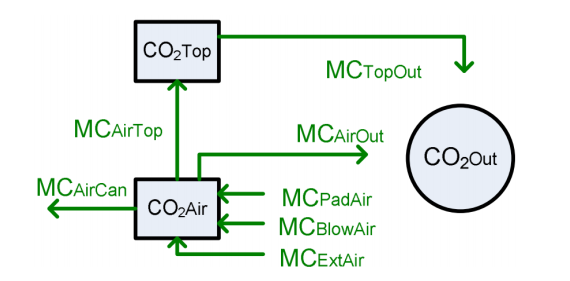
\includegraphics[scale=.5]{picture4.png}
	            \caption{Dòng chuyển động của khí $CO_2$ bên trong và bê ngoài nhà kính}
	            \label{fig:my_label}
	        \end{figure}
	    \end{center}
	    Sự thay đổi nồng độ của khí $CO_2$ ở gian trên và gian dưới được biểu diễn qua hệ gồm 2 phương trình sau đây:\\
	    \begin{cases}
            $cap_{CO_{2 Air}}\dot{CO_{2 Air}} = MC_{BlowAir} + MC_{ExtAir} + MC_{PadAir} - MC_{AirCan} - MC_{AirTop} - MC_{AirOut}$, \\
            $cap_{CO_{2 Top}}\dot{CO_{2 Top}} = MC_{AirTop} - MC_{TopOut}$
	    \end{cases}\\
	    
	    \vspace
	    
	    Trong hệ này, một số giả thiết sau được đưa ra:
	    \begin{itemize}
	        \item Lượng khí $CO_2$ ở gian trên và gian dưới không bị ảnh hưởng bởi nguồn nào khác trong những nguồn ở hình 1.
	        \item Nồng độ $CO_2$ phân bố đều nhau ở gian dưới và gian trên.
	    \end{itemize}
	    Sau đây chúng tôi sẽ trình bày một số công thức để tính $MC_{AB}$.\\
	    Đầu tiên là công thức tính lượng khí đi từ máy sưởi và gian dưới nhà kính:
	    \begin{center}
	        $MC_{BlowAir} = \dfrac{\eta_{HeatCO_2}U_{Blow}P_{Blow}}{A_{Flr}}.$
	    \end{center}
	    Trong đó:
	    \begin{itemize}
	        \item $\eta_{HeatCO_2}$ là lượng khí$CO_2$ sinh ra khi 1 Joule nhiệt lượng (cảm nhận được) được sinh ra bới máy sưởi ($mg_{CO_2}J^{-1}$).
	        \item $U_{Blow}$ thể hiện mức cho phép lượng khí $CO_2$ được sinh ra đi vào gian dưới và được điều chỉnh trong khoảng $[0,1]$.
	       \item $P_{Blow}$ là khả năng sinh ra $CO_2$ của máy sưởi (W).
	       \item $A_{Flr}$ là diện tích nhà kính ($m^2$).
	    \end{itemize}
	    \vspace{5mm}
	    Lượng khí $CO_2$ được bơm vào nhà kính bởi bên thứ 3 chuyên cung cấp khí $CO_2$ được cho bởi công thức:
	    \begin{center}
	        $MC_{ExtAir} = \dfrac{U_{ExtCO_2}\phi_{ExtCO_2}}{A_{Flr}}.$
	    \end{center}
	    Trong đó:
	    \begin{itemize}
	        \item $U_{ExtCO_2}$ là tham số điều chỉnh tốc độ bơm khí $CO_2$ vào tronh nhà kính.
	       \item $\phi_{ExtCO_2}$ là khả năng bơm $CO_2$ của bên thứ 3 ($mg s^{-1}$).
	    \end{itemize}
	    \vspace{5mm}
	    Lượng khí đi qua hệ thống thông gió vào nhà kính được tính bởi công thức sau:
	    \begin{center}
	        $MC_{PadAir} = f_{Pad}(CO_{2Out} - CO_{2Air}) = \dfrac{U_{Pad}\phi_{Pad}}{A_{Flr}}(CO_{2Out}-CO_{2Air}).$
	    \end{center}
	    Trong đó:
	    \begin{itemize}
	        \item Tốc độ đi qua tấm thông gió $f_{Pad}$ (ms$^{-1}$).
	        \item $U_{Pad}$ là mức cho phép lượng khí $CO_2$ đi qua tấm thông gió điều chỉnh được trong khoảng $[0,1]$.
	        \ỉtem $\phi_{Pad}$ là khả năng cho phép khí $CO_2$ đi qua tấm thông gió (m$^3$s$^{-1}$). 
	    \end{itemize}
	    \vspace{5mm}
	    Lượng khí đi từ gian dưới lên gian trên nhà kính được tính bởi công thức:
	    \begin{center}
	        $MC_{AirTop} = f_{ThScr}(CO_{2Air} - CO_{2Top}),$
	    \end{center}
	    Trong đó tốc độ lưu thông khí $CO_2$ qua màn chắn nhiệt $f_{ThScr}$ (m s$^{-1}$) được tính bởi:
	    \begin{center}
	        $f_{ThrScr} = U_{ThScr}K_{ThScr}\vert T_{Air}-T_{Top}\vert^{\frac{2}{3}} + (1 - U_{ThScr})\left[\dfrac{g(1-U_{ThScr})}{2\rho^{Mean}_{Air}}\vert \rho_{Air} - \rho_{Top} \vert \right]^{\frac{1}{2}}.$
	    \end{center}
	    Trong đó:
	    \begin{itemize}
	        \item $U_{ThScr} \in [0,1]$ là nơi có màn chắn nhiệt.
	        \item $T_{Top}$ (K) và $T_{Air}$ (K) lần lượt là nhiệt độ bên trên và bên dưới màn chắn.
	        \item $K_{ThScr}$ (mK$^{-\frac{2}{3}}$s$^{-1}$) là khả năng cho không khí thẩm thấu của màn chắn.
	        \item $\rho_{Air}$ và $\rho_{Top}$ (kgm$^{-3}$) lần lượt là mật độ không khí của tằng dưới và tầng trên màn chắn nhiệt.
	        \item $g$ (ms$^{-2}$) là gia tốc trọng trường.
	    \end{itemize}
	    \vspace{5mm}
	    
	    Công thức Navier-Stokes xét mô hình lý thuyết về sự trao đổi không khí thông qua các vết nứt trên bề mặt màn chắn gây ra bởi sự chênh lệch nhiệt độ không khí:
	    \begin{center}
	        $\phi_{crack} = \dfrac{L\cdot SO}{\rho_{mean}}\left[\dfrac{1}{2}\rho_{mean}\cdot SO \cdot g \cdot (\rho_{1} - \rho_{2})\right]^{\frac{1}{2}}$
	    \end{center}
	    Trong đó:
	    \begin{itemize}
	        \item $\phi_{crack}$ (m$^3$s$^{-1}$) là lưu lượng không khí đi qua màn chắn.
	        \item $L$ (m) là chiều dài khoản mở trên màn chắn.
	        \item $SO$ (m) là khoản mở trên màn chắn.
	        \item $\rho_{1}$ và $\rho_{2}$ (kgm$^{-3}$) lần lượt là mật độ phía trên và phía dưới màn chắn.
	        \item $\rho_{mean}$ (kgm$^{-3}$) là mật độ trung bình của mật độ phía trên và phía dưới.
	        \item $g$ (ms$^{-2}$) là gia tốc trọng trường.
	    \end{itemize}
	    
	    \vspace{5mm}
	    
	    Lượng khí $CO_2$ từ bên trong ra bên ngoài nhà kính theo hai hướng từ
        gian dưới và từ gian trên qua các ô thông gió ta sử dụng các công thức như dưới đây:
        \begin{center}
            $MC_{AirOut} = (f_{VentSide} + f_{VentForced})(CO_{2Air} - CO_{2Out}).$
        \end{center}
        Trong đó:
        \begin{itemize}
            \item $f_{VentSize}$ (ms$^{-1}$) là tốc độ gió từ hệ thống quạt trên tường bao xung quanh nhà kính.
            \item $f_{VentForced}$ (ms$^{-1}$)  là tốc độ gió từ hệ thống quạt bên trong nhà kính.
        \end{itemize}
    \vspace{5mm}
    Công thức tổng quát dưới đây $f_{VentRoofSide}$ (ms$^{-1}$) được dùng để thiết lập công thức cho $f_{VentSide}$:
    \begin{center}
        $f_{VentRoofSide} = \dfrac{C_d}{A_{Flr}} $
        $\bigg[ \dfrac{U_{Roof}^2U^2_{Side}A_{Roof}^2A^2_{Side}}{U^2_{Roof}A^2_{Roof} + U^2_{Side}A^2_{Side}} \cdot \dfrac{2gh_{SideRoof}(T_{Air} - T_{Out})}{T^{Mean}_{Air}} $\\
        $+ \left( \dfrac{U_{Roof}A_{Roof} + U_{Side}A_{Side}}{2} \right) ^2C_w v^2_{Wind} \bigg]$ $^{\frac{1}{2}}.$\\
        
    \end{center}
    Trong đó:
    \begin{itemize}
        \item $C_{d}$ là lưu lượng gió 
        \item $A_{Flr}$ (m$_2$) diện tích nhà kính
        \item $A_{Roof}$ (m$_2$) diện tích ô thông gió trên mái nhà
        \item $v_{Wind}$ (ms$^{-1}$) là tốc độ gió tự nhiên 
        \item $C_w$ là hệ số áp suất
    \end{itemize}
    
    \vspace{5mm}
    Khi có lười chắn côn trùng, tốc độ chuyển động của luồng khí qua các nơi thông gió sẽ giảm xuống với hệ số
    \begin{center}
        $\eta_{InsScr} = \zeta_{InsScr}(2 - \zeta_{InsScr})$
    \end{center}
    Trong đó:
    \begin{itemize}
        \item $\zeta_{InsScr}$ là độ rỗ của lưới hay tỉ lệ diện tích các lỗ trên lưới và tổng diện tích của lưới
    \end{itemize}
    
    \vspace{5mm}
    
    Tốc độ của trao đổi không khí xấp xỉ 50\% tốc độ:
    \begin{center}
        $f_{leakage} = $
        \begin{cases}
            $0.25 \cdot c_{leakage}, $ & $v_{Wind} < 0.25,$ \\
            $v_{Wind} \cdot c_{leakage}, $ & $v_{Wind} \ge 0.25.$
        \end{cases}
    \end{center}
    
    \vspace{5mm}
    
    Ta có công thức tính tốc độ gió của hệ thống quạt trên tường bao xung quanh nhà kính:
    \begin{center}
        $f_{VentSide} = $
        \begin{cases}
            $\eta_{InsScr}f^{"}_{VentSide} + 0.5f_{leakage},$ & $\eta_{Side} \ge \eta_{Side\_Thr},$\\
            $\eta_{InsScr} [ U_{ThScr}f^{"}_{VentSide}$ \\
            \hspace{1cm} $+ (1 - U_{ThScr})f_{VentRoofSide}\eta_{Side} ] + 0.5f_{leakage}, $ & $\eta_{Side} < \eta_{Side\_Thr}.$
        \end{cases}
    \end{center}
    Trong đó, $f^{"}_{VentSide}$ là $f_{VentRoofSide}$ tính tại $A_{Roof} = 0$.
    
    \vspace{5mm}
    
    Tốc độ $f_{VentForced}$ bởi hệ thống quạt gió được tính bới công thức:
    \begin{center}
        $f_{VentForced} = \dfrac{\eta_{InsScr}U_{VentForced}\phi_{VentForced}}{A_{Flr}}.$
    \end{center}
    
    Trong đó:
    \begin{itemize}
        \item $U_{VentForced}$ thể hiện sự điều chỉnh tốc độ gió cúa hệ thống và có giá trị trong khoảng $[0,1]$.
    \end{itemize}
    
    \vspace{5mm}
    
    Ta có $MC_{AirOut}$ là lượng khí $CO_2$ đi từ gian trên nhà kính ra ngoài thông qua ô mở trên mái nhà kính được tính bởi công thức:
    \begin{center}
        $MC_{TopOut} = f_{VentRoof}(CO_{2Top} - CO_{2Out}).$
    \end{center}
    
    Trong đó, $f_{VentRoof}$ là tốc độ luồng khí đi qua ô mở mái nhà kính được tính bởi công thức:
    \begin{center}
        $f_{VentRoof} = $
        \begin{cases}
            $\eta_{InsScr}f^"_{VentRoof} + 0.5f_{leakage},$ & $\eta_{Roof} \ge \eta_{Roof\_Thr},$ \\
            $\eta_{InsScr}[U_{ThScr}f^"_{VentRoof}$ \\
            \hspace{1cm} $+ (1 - U_{ThScr})f_{VentRoofSide}\eta_{Side}] + 0.5f_{leakage},$ & $\eta_{Roof} < \eta_{Roof\_Thr}.$
        \end{cases}
    \end{center}
    
    Trong trường hợp $\eta_{Roof}$ vượt ngưỡng $\eta_{Roof\_Thr}$, $^"f_{VentRoof}$ được tính như sau;
    \begin{center}
        $f^"_{VentRoof} = \dfrac{C_dU_{Roof}A_{Roof}}{2A_{Flr}}$
        $\left[ \dfrac{gh_{Roof}(T_{Air} - T_{Out})}{2T^{Mean}_{Air}} + C_wv^2_{Wind} \right]^{\frac{1}{2}}.$
    \end{center}
    
    \vspace{5mm}
    
    Lượng khí $CO_2$ bị hấp thụ vào trong tán lá thông qua quá trình quang hợp:
    \begin{center}
        $MC_{AirCan} = M_{CH_2O}h_{C_{Buf}}(P - R).$
    \end{center}
    
    Trong đó:
    \begin{itemize}
        \item $M_{CH_2O}$ là khối lượng mol $CH_2O$ (mg$\mu$ mol$^{-1}$)
        \item $P$ là tốc độ quang hợp ($\mu$mol$\{CO_2\}$m$^{-2}$s$^{-1}$)
        \item $R$ là tốc độ hô hấp của cây ($\mu$mol$\{CO_2\}$m$^{-2}$s$^{-1}$)
        \item $h_{C_{Buf}}$ là hệ số được cho bởi:
        \begin{center}
            $h_{C_{Buf}} = $
            \begin{cases}
                $0,$ & $C_{Buf} > C^{Max}_{Buf},$ \\
                $1,$ & $C_{Buf} \le C^{Max}_{Buf},$
            \end{cases}
        \end{center}
    \end{itemize}
    
    Quá trình quang hợp của lá được cho bởi định luật Fick:
    \begin{center}
        $P = \dfrac{CO_{2Air} - CO_{2Stom}}{Res}$
    \end{center}
    
    Trong đó:
    \begin{itemize}
        \item $CO_{2Stom}$ là nồng độ khí $CO_2$ hấp thụ vào trong khí khổng ($\mu$mol m$^{-3}$).
        \item $Res$ là hệ số cản trở sự hấp thụ $CO_2$ và bên trong  lá (s m$^{-1}$).
    \end{itemize}
    
    Quá trình quang hợp ở pha tối được biểu diễn qua mô hình động lực  Michaelis–Menten, khi đó tốc độ phản ứng được cho bởi công thức:
    \begin{center}
        $P = \dfrac{P_{Max} \cdot CO_{2Stom}}{CO_{2Stom} + CO_{2 \; 0.5}}$
    \end{center}
    Trong đó:
    \begin{itemize}
        \item $CO_{2 \; 0.5}$ là nồng độ khí $CO_2$ trong chất nền khi $P = P_{Max/2}$ ($\mu$mol$^{-3}$).
    \end{itemize}
    Giải tìm $CO_{2Stom}$ thì ta có tốc độ quang hợp P thỏa phương trình:
    \begin{center}
        $ResP^2 - (CO_{2 \; Air} + CO_{2\;0.5} + ResP_{Max})P + CO_{2\;Air}P_{Max} = 0$
    \end{center}
    Đối với phương trình bậc 2 trên, ta chỉ quan tâm đến nghiệm $P$ sao cho $P\rightarrow P_{Max}$ khi $CO_{2\;Air}\rightarrow+\infty$.
    
    Để giải phương trình trên, tốc độ quang hợp cực đại cần được xác định. Tốc độ đó được xác định bởi mô hình phản ứng hóa học Arrhenius
    \begin{center}
        $k(T) = k(T_0)e^{-\frac{H_a}{R}\left(\frac{1}{T} - \frac{1}{T_0}\right)}$
    \end{center}
    Trong đó:
    \begin{itemize}
        \item $k(T)$ là tốc độ phản ửng tại nhiệt độ $T$(K)
        \item $T_0$ là nhiệt độ tối ưu mà tốc độ phản ứng đã biết(K)
        \item $H_a$ là năng lượng hoạt hóa phản ứng (J\;mol$^{-1}$)
        \item $R$ là hằng số khí lí tưởng (J\;mol$^{-1}$K$^{-1}$)
    \end{itemize}
    Tuy nhiên đến một nhiệt độ càng cao đến một ngưỡng nào đó hoạt động của enzyme bị ức chế và tốc độ phản ứng sẽ giảm. Khi đó, mô hình Arrhenius không đủ để giải thích sự ức chế của enzyme và mô hình sau được xem như là mô hình cho sự hoạt động của enzyme trong quá trình quang hợp và phụ thuộc vào nhiệt độ của lá.
    \begin{center}
        $f(T) = \dfrac{1 + e^{-\frac{H_d}{R}\left(\frac{1}{T_0} - \frac{1}{\frac{H_d}{S}}\right)}}{1 + e^{-\frac{H_d}{R}\left(\frac{1}{T} - \frac{1}{\frac{H_d}{S}}\right)}}$
    \end{center}
    Trong đó:
    \begin{itemize}
        \item $f(T)$ đại diện cho sự hoạt động của enzyme ở nhiệt độ $T$(K) 
        \item $H_d$ là năng lượng ức chế enzyme (J mol$^{-1}$)
        \item $S$ là một đại lượng entropy tương ứng (J mol$^{-1}$K$^{-1}$)
    \end{itemize}
    Kết hợp hai mô hình trên, tốc độ quang hợp tối đa trên mỗi đơn vị lá được cho bởi công thức
    \begin{center}
        $P_{Max}(T) = k(T)f(T)$
    \end{center}
    
    \vspace{5mm}
    
    Ta có định luật Beer về sự hấp thụ ánh sáng của tán lá dưới sự ảnh hưởng của chỉ số $LAI$ (leaf area index).
    \begin{center}
        $I = \dfrac{I_0.K.e^{-K.LAI}}{1 - m}$
    \end{center}
    Trong đó:
    \begin{itemize}
        \item $I_0$ là năng lượng ánh sáng đi đến tán lá trước khi vào tán lá ($\mu$mol \{photon\} m$^{-2}$s$^{-1}$)
        \item $I$ là năng lượng ánh sáng sai khi đi xuyên qua tán lá ($\mu$mol \{photon\} m$^{-2}$s$^{-1}$)
        \item $K$ là hệ số tắt có giá trị từ 0.7 tới 1.0 nếu lá cây phân tầng ngang như cây cà chua và từ 0.3 đến 0.5 nếu lá cây nằm nghiêng như trong trường hợp cây lúa nước
        \item $m$ là hệ số truyền ánh sáng của lá cây và thường mặc định là 0.1
    \end{itemize}
    Khi đó năng lượng ánh sáng mà lá cây nhận được là sự chênh lệch năng lượng của tia trước khi vào tán là và tia ló sau khi vào tán lá và được tính bởi công thức
    \begin{center}
        $L = L_0 \left(1 - \dfrac{K.e^{-K.LAI}}{1 - m}\right)$
    \end{center}
    Trong đó:
    \begin{itemize}
        \item $L$ là lượng photon nhận được bởi lá cây ($\mu$mol \{photon\} m$^{-2}$s$^{-1}$)
        \item $L_0$ là lượng photon ban đầu phía trên tán lá ($\mu$mol \{photon\} m$^{-2}$s$^{-1}$)
    \end{itemize}
    
    Sau đây ta có công thức Arrhenius mở rộng thay cho công thức Arrhenius ở trên
    \begin{center}
        $k(T) = LAI.k(T_0).e^{-\frac{H_d}{R}\left(\frac{1}{T_0} - \frac{1}{\frac{H_d}{S}}\right)}$
    \end{center}.
    
    \vspace{5mm}
    
    Khác với mô hình quang hợp cho một đơn vị lá, lượng năng lượng ánh sáng hấp thụ vào trong tán lá bị ảnh hưởng bởi LAI cần được thêm vào và ảnh hưởng đến tốc độ quang hợp cực đại $P_{Max}$. Do đó, ta xét mô hình sau cho $P_{Max}$, là hàm số phụ thuộc vào $L$ và $T$.
    
    \begin{center}
        $P_{Max}(L, T) = \dfrac{P_{MLT}.P_{Max}(T).L}{L + L_{0.5}}$
    \end{center}
    Trong đó:
    \begin{itemize}
        \item $L_{0.5}$ là lượng ánh sáng khi $P_{Max}(L,T) = P_{Max}(T/2)$ ($\mu$mol \{photon\} m$^{-2}$s$^{-1}$)
        \item $P_{MLT}$ là tốc độ quang hợp cực đại tại điểm bão hòa ánh sáng và nhiệt độ tối ưu $T$.
    \end{itemize}
\subsubsection{Code bài 2b}
\textbf{Dữ liệu được đọc từ file $data\_in\textbackslash data\_CO2.xlsx$} \\
\text{Source trích từ file $source\textbackslash code2\_4.py$}
\begin{minted}{python}
import math
from math import sqrt
import pandas as pd
from xlsxwriter import Workbook

# formula 3
def cal_MCBlowAir(nHeatCO2, UBlow, PBlow, AFlr):
    return nHeatCO2 * UBlow * PBlow / AFlr


# formula 4
def cal_MCExtAir(UExtCO2, phiExtCO2, AFlr):
    return UExtCO2 * phiExtCO2 / AFlr


# formula 5
def cal_MCPadAir_1(fPad, CO2Out, CO2Air):
    return fPad * (CO2Out - CO2Air)


def cal_MCPadAir_2(UPad, phiPad, AFlr, CO2Out, CO2Air):
    fPad = UPad * phiPad / AFlr
    return fPad * (CO2Out - CO2Air)


# formula 6
def cal_MCAirTop(fThScr, CO2Air, CO2Top):
    return fThScr * (CO2Air - CO2Top)


# formula 7
def cal_fThScr(UThScr, KThScr, TAir, TTop, g, pAir, pTop):
    a = UThScr * KThScr * pow(abs(TAir - TTop), 2 / 3)
    PMean_Air = (pAir + pTop) / 2
    b = (1 - UThScr) * pow(g * (1 - UThScr) * abs(pAir - pTop) / (2 * PMean_Air), 1 / 2)
    return a + b


# formula 9
def cal_MCAirOut(fVentSide, fVentForce, CO2Air, CO2Out):
    return (fVentSide + fVentForce) * (CO2Air - CO2Out)


# formula 10
def cal_ppfVentRoofSide(Cd, AFlr, URoof, USide, ARoof, ASide, g, hSideRoof, TAir, TOut, Cw, vWind):
    a = Cd / AFlr
    b = pow(URoof * USide * ARoof * ASide, 2) / (pow(URoof * ARoof, 2) + pow(USide * ASide, 2))
    TMean_Air = (TAir + TOut) / 2
    c = 2 * g * hSideRoof * (TAir - TOut) / TMean_Air
    _d = (URoof * ARoof + USide * ASide) / 2
    d = pow(_d, 2) * Cw * pow(vWind, 2)
    return a * sqrt(b * c + d)


# formula 11
def cal_nInsScr(sInsScr):
    return sInsScr * (2 - sInsScr)


# formula 12
def cal_fleakage(cleakage, vWind):
    if vWind < 0.25:
        return 0.25 * cleakage
    else:
        return vWind * cleakage


# formula (**) calculate ppfVentSide
def cal_ppfVentSide(Cd, USide, ASide, vWind, AFlr, Cw):
    return Cd * USide * ASide * vWind * sqrt(Cw) / (2 * AFlr)


# formula 13, use formula 10 and formula (**)
def cal_fVentSide(nInsScr, ppfVentSide, fleakage, UThScr, ppfVentRoofSide, nSide, nSide_Thr):
    # nSide_Thr la nguong Stack
    # pp_fVentSide la f"VentSide tinh bang ppfVentRoofSide tai ARoof = 0
    if nSide >= nSide_Thr:
        return nInsScr * ppfVentSide + 0.5 * fleakage
    else:
        return nInsScr * (UThScr * ppfVentSide + (1 - UThScr) * ppfVentRoofSide * nSide) + 0.5 * fleakage


# formula 14
def cal_fVentForced(nInsScr, UVentForced, phiVentForced, AFlr):
    return nInsScr * UVentForced * phiVentForced / AFlr


# formula 15
def cal_MCTopOut(fVentRoof, CO2Top, CO2Out):
    return fVentRoof * (CO2Top - CO2Out)


# formula 16
def cal_fVentRoof(nInsScr, fleakage, UThScr, ppfVentRoofSide, nRoof, nSide, nRoof_Thr, ppfVentRoof):
    # nRoof_Thr la nguong Stack
    if nRoof >= nRoof_Thr:
        return nInsScr * ppfVentRoof + 0.5 * fleakage
    else:
        return nInsScr * (UThScr * ppfVentRoof + (1 - UThScr) * ppfVentRoofSide * nSide) + 0.5 * fleakage


# formula 17
def cal_ppfVentRoof(Cd, URoof, ARoof, AFlr, g, hVent, TAir, TOut, Cw, vWind):
    TMeanAir = (TAir + TOut) / 2
    part1 = Cd * URoof * ARoof / (2 * AFlr)
    part2 = g * hVent * (TAir - TOut) / 2 / TMeanAir + Cw * pow(vWind, 2)
    return part1 * sqrt(part2)


# formular 18 include 19
# tinh P
def cal_P(CO2Air, LAI):
    T_Can_K = 20 + 273
    J_POT = LAI * 210 * math.exp(37000 * (T_Can_K - 298.15) / (8.314 * T_Can_K * 298.15)) * (
                1 + math.exp((710 * 298.15 - 220000) / (8.314 * 298.15))) / (
                        1 + math.exp((710 * T_Can_K - 220000) / (8.314 * T_Can_K)))
    J = (J_POT + 38.5 - math.sqrt(math.pow(J_POT + 38.5, 2) - 2.8 * J_POT * 38.5)) / 1.4
    CO2Stom = 0.67 * CO2Air
    P = (J * (CO2Stom - 498.1)) / (4 * (CO2Stom + 2 * 498.1))
    return P


# tinh R
def cal_R(CO2Air, P):
    CO2Stom = 0.67 * CO2Air
    R = P * 498.1 / CO2Stom
    return R


def cal_MCAirCan(P, R, CBuf, CMaxBuf):
    MCH2O = 0.03
    hCBuf = 1
    if CBuf > CMaxBuf:
        hCBuf = 0
    return MCH2O * hCBuf * (P - R)

print("Input line of data")
i = int(input())
# Read data from excel file
data = pd.read_excel("../data_in/data_CO2.xlsx")
df = pd.DataFrame(data)
nHeatCO2 = float(df.at[i, "nHeatCO2"])
UBlow = float(df.at[i, "UBlow"])
PBlow = float(df.at[i, 'PBlow'])
AFlr = float(df.at[i, 'AFlr'])
UExtCO2 = float(df.at[i, 'UExtCO2'])
phiExtCO2 = float(df.at[i, 'phiExtCO2'])
UPad = float(df.at[i, 'UPad'])
phiPad = float(df.at[i, 'phiPad'])
CO2Out = float(df.at[i, 'CO2Out'])
LAI = float(df.at[i, 'LAI'])
CBuf = float(df.at[i, 'CBuf'])
CMax_Buf = float(df.at[i, 'CMax_Buf'])
UThScr = float(df.at[i, 'UThScr'])
KThScr = float(df.at[i, 'KThScr'])
TAir = float(df.at[i, 'TAir'])
TTop = float(df.at[i, 'TTop'])
g = float(df.at[i, 'g'])
pAir = float(df.at[i, 'pAir'])
pTop = float(df.at[i, 'pTop'])
cleakage = float(df.at[i, 'cleakage'])
vWind = float(df.at[i, 'vWind'])
Cd = float(df.at[i, 'Cd'])
URoof = float(df.at[i, 'URoof'])
USide = float(df.at[i, 'USide'])
ARoof = float(df.at[i, 'ARoof'])
ASide = float(df.at[i, 'ASide'])
hSideRoof = float(df.at[i, 'hSideRoof'])
TOut = float(df.at[i, 'TOut'])
Cw = float(df.at[i, 'Cw'])
nSide = float(df.at[i, 'nSide'])
nSide_Thr = float(df.at[i, 'nSide_Thr'])
sInsScr = float(df.at[i, 'sInsScr'])
UVentForced = float(df.at[i, 'UVentForced'])
phiVentForced = float(df.at[i, 'phiVentForced'])
capCO2Air = float(df.at[i, 'capCO2Air'])
hVent = float(df.at[i, 'hVent'])
nRoof = float(df.at[i, 'nRoof'])
nRoof_Thr = float(df.at[i, 'nRoof_Thr'])
capCO2Top = float(df.at[i, 'capCO2Top'])
CO2Air = float(df.at[i, 'CO2Air'])
CO2Top = float(df.at[i, 'CO2Top'])

# formular 1
def dxCO2Air(CO2Air, CO2Top):
    # TODO

    ######## Calculate MCBlowAir ########
    MCBlowAir = cal_MCBlowAir(nHeatCO2, UBlow, PBlow, AFlr)
    print("MCBlowAir = ", MCBlowAir)
    ######## Calculate MCExtAir ########
    MCExtAir = cal_MCExtAir(UExtCO2, phiExtCO2, AFlr)
    print("MCExtAir = ", MCExtAir)
    ######## Calculate MCPadAir ########
    MCPadAir = cal_MCPadAir_2(UPad, phiPad, AFlr, CO2Out, CO2Air)
    print("MCPadAir = ", MCPadAir)
    ######## Calculate MCAirCan ########
    P = cal_P(CO2Air, LAI)
    R = 0
    MCAirCan = cal_MCAirCan(P, R, CBuf, CMax_Buf)
    print("MCAirCan = ", MCAirCan)
    ######## Calculate MCAirTop ########
    fThScr = cal_fThScr(UThScr, KThScr, TAir, TTop, g, pAir, pTop)
    MCAirTop = cal_MCAirTop(fThScr, CO2Air, CO2Top)
    print("MCAirTop = ", MCAirTop)
    ######## Calculte MCAirOut ########
    # Calculate fleakage
    fleakage = cal_fleakage(cleakage, vWind)

    # Calculate ppfVentRoofSide
    ppfVentRoofSide = cal_ppfVentRoofSide(Cd, AFlr, URoof, USide, ARoof, ASide, g, hSideRoof, TAir, TOut, Cw, vWind)

    # Calculate ppfVentSide
    ppfVentSide = cal_ppfVentSide(Cd, USide, ASide, vWind, AFlr, Cw)

    # Calculate fVentSide
    nInsScr = cal_nInsScr(sInsScr)
    fVentSide = cal_fVentSide(nInsScr, ppfVentSide, fleakage, UThScr, ppfVentRoofSide, nSide, nSide_Thr)

    # Calculate fVentForce
    fVentForced = float(cal_fVentForced(nInsScr, UVentForced, phiVentForced, AFlr))

    MCAirOut = cal_MCAirOut(fVentSide, fVentForced, CO2Air, CO2Out)
    print("MCAirOut = ", MCAirOut)
    return (MCBlowAir + MCExtAir + MCPadAir - MCAirCan - MCAirTop - MCAirOut) / capCO2Air


# formula 2
def dxCO2Top(CO2Air, CO2Top):
    # TODO

    ######## Calculate MCAirTop ########
    fThScr = cal_fThScr(UThScr, KThScr, TAir, TTop, g, pAir, pTop)
    MCAirTop = cal_MCAirTop(fThScr, CO2Air, CO2Top)
    print("MCAirTop = ", MCAirTop)
    ######## Calculate MCTopOut ########
    # Calculate ppfVentRoofSide
    ppfVentRoofSide = cal_ppfVentRoofSide(Cd, AFlr, URoof, USide, ARoof, ASide, g, hSideRoof, TAir, TOut, Cw, vWind)

    # Calculate ppfVentRoof
    ppfVentRoof = cal_ppfVentRoof(Cd, URoof, ARoof, AFlr, g, hVent, TAir, TOut, Cw, vWind)

    # Calculate fleakage
    fleakage = cal_fleakage(cleakage, vWind)

    # Calculate fVentRoof
    nInsScr = cal_nInsScr(sInsScr)
    fVentRoof = cal_fVentRoof(nInsScr, fleakage, UThScr, ppfVentRoofSide, nRoof, nSide, nRoof_Thr, ppfVentRoof)
    MCTopOut = cal_MCTopOut(fVentRoof, CO2Top, CO2Out)
    print("MCTopOut = ", MCTopOut)

    return (MCAirTop - MCTopOut) / capCO2Top

\end{minted}
\subsection{Bài 3: Chạy thử một số dữ liệu}
\begin{minted}{python}
print("dxCO2Air = ", dxCO2Air(CO2Air, CO2Top))
print("dxCO2Top = ", dxCO2Top(CO2Air, CO2Top))
\end{minted}
\begin{itemize}
    \item Với data đọc từ dòng $0$ của data\_CO2.xlsx trong thư mục data\_in, ta có kết quả sau:\\
    Input line of data: \\
    0\\
    MCBlowAir =  0.20357142857142857\\
    MCExtAir =  4.628571428571429\\
    MCPadAir =  0.006727714285714286\\
    MCAirCan =  -0.037749295986342614\\
    MCAirTop =  0.0\\
    MCAirOut =  -0.04095714285714286\\
    dxCO2Air =  0.8195961683786762\\
    MCAirTop =  0.0\\
    MCTopOut =  -0.027457624285367757\\
    dxCO2Top =  0.013728812142683879\\
    \item Với data đọc từ dòng $1$ của data\_CO2.xlsx trong thư mục data\_in, ta có kết quả sau:\\
    Input line of data: \\
    1\\
    MCBlowAir =  1.8321428571428573\\
    MCExtAir =  4.628571428571429\\
    MCPadAir =  0.006727714285714286\\
    MCAirCan =  -0.037749295986342614\\
    MCAirTop =  0.0\\
    MCAirOut =  -0.04095714285714286\\
    dxCO2Air =  1.0910247398072477\\
    MCAirTop =  0.0\\
    MCTopOut =  -0.027457624285367757\\
    dxCO2Top =  0.013728812142683879\\
\end{itemize}


\subsection{Bài 4}
Source trích từ $source\textbackslash code2\_4.py$\\
\textbf{a)} Dựa trên cơ sở lý thuyết của phương phép Euler và Runge-Kutta bậc 4 đã nêu ở trên, chúng tôi đã tạo ra các Solver chạy bằng ngôn ngữ Python để dự đoán kết quả của mô hình.\\
Với các tham số đầu vào là $CO2Air$(giá trị tại thời điểm t của CO2Air), $CO2Top$(giá trị tại thời điểm t của CO2Top), $h$(kích thước bước sấp xỉ), $time$(thời điểm t cần tính giá trị của CO2Air và CO2Top)

\begin{minted}{python}
def euler(CO2Air, CO2Top, h, time):
    n = int(time/h)
    CO2Air_0 = CO2Air
    CO2Top_0 = CO2Top

    for idx in range(1, n + 1):
        k = h * dxCO2Air(CO2Air_0, CO2Top_0)
        t = h * dxCO2Top(CO2Air_0, CO2Top_0)

        CO2Air_0 += k
        CO2Top_0 += t

        if idx % 300 == 0:
            row = idx // 300
            worksheet.write(row + 1, 0, idx)
            worksheet.write(row + 1, 1, CO2Air_0)
            worksheet.write(row + 1, 2, CO2Top_0)
            global TAir, TTop, TOut, vWind, URoof
            TAir = float(df.at[row, 'TAir'])
            TTop = float(df.at[row, 'TTop'])
            TOut = float(df.at[row, 'TOut'])
            vWind = float(df.at[row, 'vWind'])
            URoof = float(df.at[row, 'URoof'])

    return CO2Air_0, CO2Top_0


def rk4(CO2Air, CO2Top, h, time):
    n = int(time/h)
    CO2Air_0 = CO2Air
    CO2Top_0 = CO2Top

    for idx in range(1, n + 1):
        k1 = h * dxCO2Air(CO2Air_0, CO2Top_0)
        t1 = h * dxCO2Top(CO2Air_0, CO2Top_0)
        k2 = h * dxCO2Air(CO2Air_0+0.5*k1, CO2Top_0+0.5*k1)
        t2 = h * dxCO2Top(CO2Air_0+0.5*t1, CO2Top_0+0.5*t1)
        k3 = h * dxCO2Air(CO2Air_0+0.5*k2, CO2Top_0+0.5*k2)
        t3 = h * dxCO2Top(CO2Air_0+0.5*t2, CO2Top_0+0.5*t2)
        k4 = h * dxCO2Air(CO2Air_0+k3, CO2Top_0+k3)
        t4 = h * dxCO2Top(CO2Air_0+t3, CO2Top_0+t3)

        CO2Air_0 += (1.0/6.0) * (k1+2*k2+2*k3+k4)
        CO2Top_0 += (1.0/6.0) * (t1+2*t2+2*t3+t4)

        if idx % 300 == 0:
            row = idx // 300
            worksheet.write(row + 1, 4, CO2Air_0)
            worksheet.write(row + 1, 5, CO2Top_0)
            global TAir, TTop, TOut, vWind, URoof
            TAir = float(df.at[row, 'TAir'])
            TTop = float(df.at[row, 'TTop'])
            TOut = float(df.at[row, 'TOut'])
            vWind = float(df.at[row, 'vWind'])
            URoof = float(df.at[row, 'URoof'])

    return CO2Air_0, CO2Top_0

\end{minted}
\\
    \textit{Note: } các biến như vận tốc gió(vWind), nhiệt độ(TAir, TTop, TOut), URoof (tính thông qua ventWind và ventLee) thay đổi sau mỗi 5 phút nên cần cập nhật chúng trong quá trình tính toán .
\\\\
\textbf{b)}
Với các Solver ở trên, ta tính được giá trị xấp xỉ của $CO2Air$ và $CO2Top$ tại thời điểm t đúng 5 phút, 10 phút, 15 phút,....
\\\\
\textbf{Dữ liệu được đọc từ file $data\_in\textbackslash data\_4.xlsx$} \\
\begin{minted}{python}
############## main ##############
def main():
    print(df.at[0, 'Place'])
    print('CO2Air_0: ', CO2Air)
    print('CO2Top_0: ', CO2Top)

    step = float(input('Input step: '))
    time = float(input('Input time: '))

    air, top = euler(CO2Air, CO2Top, step, time)
    print('\nExplicit Euler')
    print('The CO2Air: ', round(air, 10))
    print('The CO2Top: ', round(top, 10))

    air, top = rk4(CO2Air, CO2Top, step, time)
    print('\nExplicit Runge-Kutta 4th order')
    print('The CO2Air: ', round(air, 10))
    print('The CO2Top: ', round(top, 10))


wb = Workbook('data_out\Output_4.xlsx')
worksheet = wb.add_worksheet()
worksheet.write(0, 0, 'time')
worksheet.write(0, 1, 'CO2Air_E')
worksheet.write(0, 2, 'CO2Top_E')
worksheet.write(0, 4, 'CO2Air_RK4')
worksheet.write(0, 5, 'CO2Top_RK4')
worksheet.write(1, 0, 0)
worksheet.write(1, 1, CO2Air)
worksheet.write(1, 2, CO2Top)
worksheet.write(1, 4, CO2Air)
worksheet.write(1, 5, CO2Top)
main()
wb.close()
\end{minted}
\\
Các tham số đầu vào được đọc từ file $data\_in\textbackslash data\_4.xlsx$. Nhập giá trị i (line of data) là 0 .Nhập kích thước bước sấp sỉ (h) là 1 (s) từ bàn phím. Nhập thời điểm t (time) là 603600 (s) tương ứng 1 tuần. Giá trị $CO2Air$ và $CO2Top$ tính được sau mỗi 300s sẽ được ghi vào file $Output\_4.xslx$.
\\\\
Với file $Output\_4.xslx$ ta tính độ chênh lệch của kết quả so với dữ liệu thật được lưu trong file $data\_4.xslx$ thông qua hàm $mse$ (mean squared error) và vẽ đồ thị.


\begin{minted}{python}
def mse(a):
    n = 0
    for idx in range(0, nRow):
        n += math.pow((float(df.at[idx, a]) - float(de.at[idx, 'CO2Air_real'])),2)
    return n/nRow

data = pd.read_excel("data_out\Output_4.xlsx")
df = pd.DataFrame(data)
da = pd.read_excel("data_in\data_4.xlsx")
de = pd.DataFrame(da)
nRow = len(df.index)

print(mse('CO2Air_E'))
print(mse('CO2Air_RK4'))
\end{minted}
\\
Kết quả là :\\
mse('CO2Air\_E') = 80342.82022615442 (độ lệch của phương pháp Euler)\\
mse('CO2Air\_RK4') = 80307.17721401696 (độ lệch của phương pháp Runge-Kutta 4)\\

Vì số liệu của các yếu tố bên trong nhà kính dùng để tính $CO2Air$ và $CO2Top$ không khớp với số liệu mà dữ liệu thật dùng để đo nên độ chính xác của mô hình không được cao. 

\begin{figure}[h]
\begin{center}
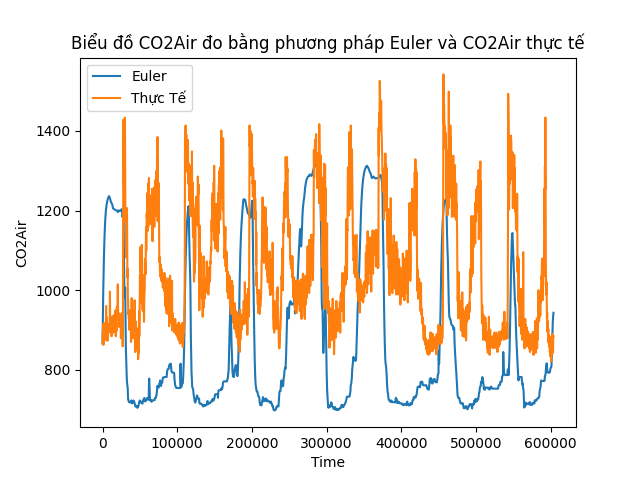
\includegraphics[width=7cm]{4b_euler.png}
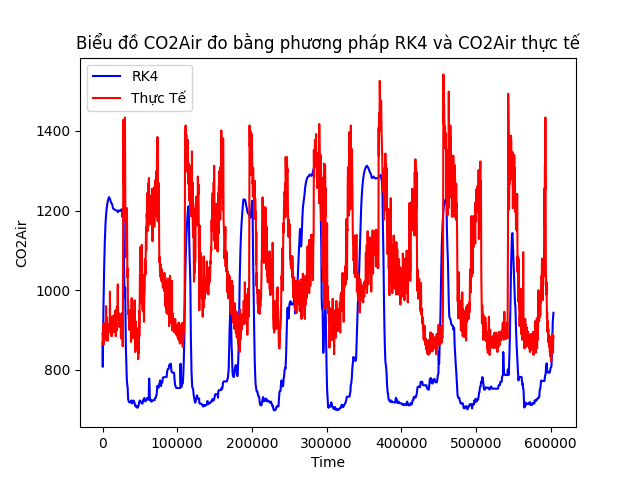
\includegraphics[width=7cm]{4b_rk4.png}
\end{center}
\end{figure}

\begin{figure}[h]
\begin{center}
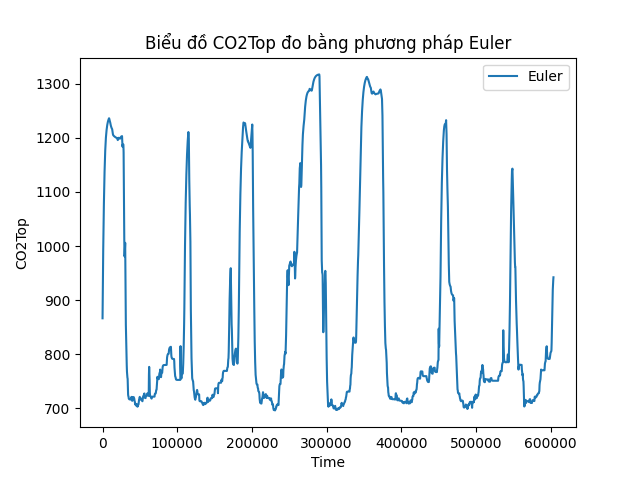
\includegraphics[width=7cm]{4b_TOP_Euler.png}
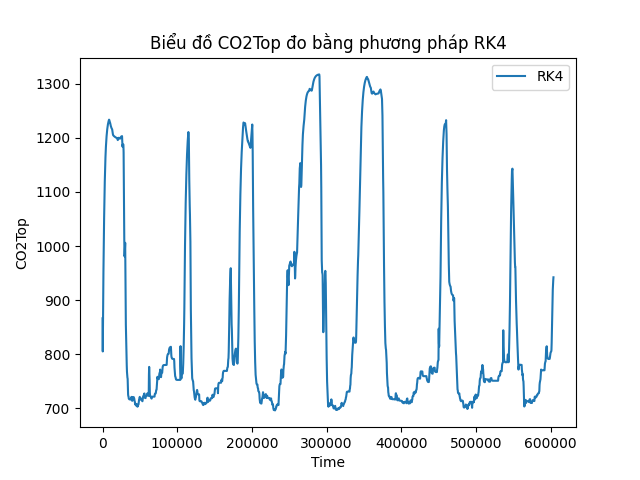
\includegraphics[width=7cm]{4b_TOP_RK4.png}
\end{center}
\end{figure}

\newpage


\subsection{Bài 5}
\subsubsection{Bài 5.2}
\subsubsubsection{Bài 5.2.a: Chi tiết mô hình đối với áp suất hơi nước $VP$ trong nhà kính được sử dụng trong đề tài này}

    Công thức biểu diễn sự thay đổi áp suất hơi nước của hơi nước như sau:\\
    \begin{cases}
        $cap_{VP_{Air}}\dot{VP_{Air}} = MV_{CanAir} + MV_{PadAir} + MV_{FogAir} + MV_{BLowAir}$\\ 
        \hspace{2.4cm} - $MV_{AirThScr} - MV_{AirTop} - MV_{AirOut\_Pad} - MV_{AirMech}$, \\
        $cap_{VP_{Top}}\dot{VP_{Top}} = MV_{AirTop} - MV_{TopCov,in} - MV_{TopOut}$
    \end{cases}\\
    
    
    
    Hệ số chuyển đổi áp suất hơi nước từ khối lượng nước trong lượng khí nằm phía dưới màn chắn nhiệt được mô tả bởi công thức:
    \begin{center}
        $cap_{VP_{Air}} = \dfrac{M_{Water}h_{Air}}{R(T_{Air} + 273.5)}$
    \end{center}
    Trong đó:
    \begin{itemize}
        \item $M_{Water}$ là khối lượng mol của nước (kg kmol $^{-1}$)
        \item $h_{Air}$ là chiều cao từ nền tới màn chắn nhiệt (m)
        \item $R$ là hằng số khí lí tưởng (J kmol$^{-1}$K$^{-1}$) 
    \end{itemize}
    Tương tự ta có công thức biểu diễn cho $cap_{VP_{Top}}$
    \begin{center}
        $cap_{VP_{Top}} = \dfrac{M_{Water}h_{Top}}{R(T_{Top} + 273.5)}$
    \end{center}
    
    \vspace{5mm}
    
    Hệ số trao đổi hơi nước giữa không khí và các đối tượng có mối quan hệ tuyến tính với hệ số trao đổi nhiệt đối lưu giữa không khí và các vật thể. Ta có công thức mô tả dòng hơi nước tới đối tượng bằng công thức:
    \begin{center}
        $MV_{12} = $
        \begin{cases}
            $0$ & $VP_1 < VP_2$ \\
            $6.4 \cdot 10^{-9} HEC_{12}(VP_1 - VP_2)$ & $VP_1 > VP_2$
        \end{cases}
        \hspace{1cm}
        $[kg m^{-2} s^{-1}]$
    \end{center}
    Trong đó:
    \begin{itemize}
        \item $MV_{12}$ là thông lượng hơi từ  không khí từ vị trí 1 đến vật thể 2 (kg m$^{-2}$ s$^{-1}$)
        \item $6.4 \cdot 10^{-9}$ là hệ số chuyển đổi liên quan hệ số trao đổi nhiệt với hệ số trao đổi hơi
        \item $HEC_{12}$ là hệ số trao đổi nhiệt giữa không khí ở vị trí 1 và đối tượng 2 (W m$^{-2}$ K$^{-1}$)
        \item $VP_1$ là áp suất hơi nước ở vị trí 1
        \item $VP_2$ là áp suất hơi nước ở vị trí 2
    \end{itemize}
    Vì mô hình chỉ nên bao gồm các phương trình vi phân, nên phương trình trên được chuyển về phương trình vi phân bằng cách sử dụng “hàm số khả vi chuyển đổi”
    \begin{center}
        $MV_{12} = \dfrac{1}{1 + exp(s_{MV_{12}}(VP_1 - VP_2))}.6.4 \cdot 10^{-9} HEC_{12}(VP_1 - VP_2)$
    \end{center}
    Trong đó:
    \begin{itemize}
        \item $s_{MV_{12}}$ là độ dốc của hàm chuyển đổi đối với sự chênh lệch áp suất hơi nước
    \end{itemize}
    Ta có thông lượng hơi nước từ gian dưới nhà kính tới màn chắn nhiệt $MV_{AirThScr}$ và từ gian trên tới lớp bao bên trong $MV_{TopCov,in}$ được tính tương tự như công thức trên.
    
    \vspace{5mm}
    
    Dạng chung cho dòng hơi nước kèm theo không khí được mô tả bới:
    \begin{center}
        $MV_{12} = \dfrac{M_{Water}}{R}.f_{12}.\left(\dfrac{VP_1}{T_1 + 273.15} - \dfrac{VP_2}{T_2 + 273.15}\right)$
    \end{center}
    Trong đó:
    \begin{itemize}
        \item $MV_{12}$ là thông lượng hơi nước từ nơi 1 tới nơi 2
        \item $f_{12}$ là thông lượng không khí từ nơi 1 tới nơi 2 (m$^3$m$^{-2}$s$^{-1}$)
        \item $T_1$ và $T_2$ là nhiệt độ ở nơi 1 và nơi 2.
    \end{itemize}
    Các dòng hơi nước $MV_{AirTop}$, $MV_{AirOut}$, $MV_{TopOut}$ được mô tả tương tự công thức trên.Theo đó, thông lượng không khí đi kèm theo chúng là $f_{ThScr}$ (thông lượng qua màn chắn nhiệt), $f_{VentSide} + f_{VentForced}$ (thông lượng gió qua cửa và cưỡng bức), $f_{VentRoof}$ là thông lượng gió trên mái.
    
    \vspace{5mm}
    
    Sự thoát hơi nước của tán lá được miêu tả bởi công thức:
    \begin{center}
        $MV_{CanAir} = VEC_{CanAir}(VP_{Can} - VP_{Air})$
    \end{center}
    Trong đó:
    \begin{itemize}
        \item $VEC_{CanAir}$ là hệ số chuyển đổi hơi nước giữa tán lá và không khí (kg Pa s$^{-1}$)
        \item $VP_{Can}$ là áp suất hơi bão hòa ở nhiệt độ tán cây
    \end{itemize}
    
    Theo Stanghellini thì hệ số chuyển đổi hơi nước giữa tán lá và không khí được tính bởi
    \begin{center}
        $VEC_{CanAir} = \dfrac{2\rho_{Air}c_{p,Air}LAI}{\Delta H \gamma(r_b + r_s)}$
    \end{center}
    Trong đó:
    \begin{itemize}
        \item $\rho_{Air}$ là mật độ không khí của nhà kính (kg m$^{-3}$)
        \item $c_{p,Air}$ là nhiệt riêng của không khí trong nhà kính (J K$^{-1}$kg$^{-1}$)
        \item $LAI$ là chỉ số diện tích lá 
        \item $\Delta H$ là nhiệt độ ngầm của sự bay hơi nước (J kg$^{-1}$)
        \item $\gamma$ là hệ số psychometric (PA K$^{-1}$)
        \item $r_b$ là sức cản của mặt trên tán lá đối với sự bay hơi (s m$^{-1}$)
        \item $r_s$ là sức cản của khí khổng đối với sự bay hơi (s m$^{-1}$)
    \end{itemize}
    
    Sức cản trở bay hơi của mặt trên lá được tính như sau:
    \begin{center}
        $r_s = r_{s, min} \cdot rf(R_{Can}) \cdot rf(CO_{2\;Air\_ppm}) \cdot 
        rf(VP_{Can} - VP_{Air})$
    \end{center}
    Trong đó:
    \begin{itemize}
        \item $r_{s, min}$ là khả năng cản trở tối thiểu  (s m$^{-1}$)
        \item $rf$ là hệ số kháng mức bức xạ cao, mức $CO_2$ cao và độ chênh lệch áp suất hơi nước cao.
    \end{itemize}
    
    Theo Stanghellinin thì hệ số kháng được tính như sau:
    \begin{center}
        $rf(R_{Can}) = \dfrac{R_{Can} + c_{evap1}}{R_{Can} + c_{evap2}}$\\
        $rf(CO_{2\;Air}) = 1 + c_{evap3}(\eta_{mg\_ppm}CO_{2Air} - 200)^2$\\
        $rf(VP_{Can} - VP_{Air}) = 1 + c_{evap4}(VP_{Can} - VP_{Air})^2$ 
    \end{center}
    Trong đó:
    \begin{itemize}
        \item $R_{Can}$ là bức xạ toàn cầu trên tán cây(W m$^{-2}$)
        \item $\eta_{mg\_ppm}$ là hệ chuyển đổi từ mg m$^{-3}$ sang ppm
        \item $c_{evap1}$ là hệ số kháng cho mức $CO_2$ cao và bằng 1.5 (Wm$^{-2}$)
        \item $c_{evap2}$ là hệ số kháng cho độ chênh lệch áp suất hơi nước ở mức cao và bằng 5.8 (Wm$^{-2}$)
    \end{itemize}
    
    Tham số $c_{evap3}$ và $c_{evap4}$ có sự thay đổi giữa ban ban ngày và ban đêm. Vì thế ta dùng một hệ số chuyển đổi để làm cho công thức có thể phân biệt được giữa ban đêm và ban ngày
    \begin{center}
        $S_{r_s} = \dfrac{1}{1 + exp(s_{r_s}(R_{Can} - R_{Can\_SP})}$
    \end{center}
    Trong đó:
    \begin{itemize}
        \item $S_{r_s}$ là giá trị của biến chuyển
        \item $s_{r_s}$ là độ dốc cuả biến chuyển trong mô hình kháng khí khổng
        (m W$^{-2}$) 
        \item $R_{Can\_SP}$ là bức xạ phía trên tán lá để xác định ngày hay đêm (Wm$^{-2}$)
    \end{itemize}
    Dùng giá trị chuyển đổi, thông số thoát hơi nước sau khi được làm mịn được mô tả bằng
    \begin{center}
        $c_{evap3} = c^{night}_{evap3}(1 - S_{r_s}) + c^{night}_{evap3}S_{r_s}$
    \end{center}
    Tham số $c_{evap4}$ cũng được tính tương tự như trên.
    
    \vspace{5mm}
    
    Dưới đây là công thức để tính $MV_{BlowAir}$ là lượng hơi nước đi từ máy sưởi vào gian dưới nhà kính
    \begin{center}
        $MV_{BlowAir} = \dfrac{\eta_{HeatVap}U_{Blow}P_{Blow}}{A_{Flr}}$
    \end{center}
    Trong đó:
    \begin{itemize}
        \item $\eta_{HeatVap}$ là lượng hơi nước được tạo ra khi 1 Juole năng lượng được tiêu thụ hoàn toàn bởi máy sưởi (kg vapour J$^{-1}$).
    \end{itemize}
    
    \vspace{5mm}
    
    Lượng hơi nước từ quạt gió vào gian dưới được tính bởi:
    \begin{center}
        $MV_{PadAir} = \rho_{Air}f_{Air}(\eta_{Pad}(x_{Pad} - x_{Out}) + x_{Out})$
    \end{center}
    Trong đó:
    \begin{itemize}
        \item $f_{Air}$ là thông lượng gió của hệ thống quạt (m$^3$m$^{-2}$s$^{-1}$)
        \item $\rho_{Pad}$ là độ mở của hệ thống quạt
        \item $x_{Pad}$ là tỉ lệ hơi nước trong không khí của cửa vào hệ thống quạt (kg water kg$^{-1}$ air)
        \item $x_{Out}$ là tỉ lệ hơi nước trong không khí của cửa ra hệ thống quạt (kg water kg$^{-1}$ air)
    \end{itemize}
    Dòng thông gió của hệ thống quạt được mô tả bằng
    \begin{center}
        $f_{Pad} = \dfrac{U_{Pad}\phi_{Pad}}{A_{Flr}}$
    \end{center}
    Trong đó:
    \begin{itemize}
        \item $U_{Pad}$ là độ mở của hệ thống quạt
        \item $\phi_{Pad}$ là sức chứa thông lượng của  khí đi qua hệ thống quạt (m$^3$s$^{-1}$)   
    \end{itemize}
    
    \vspace{5mm}
    
    Lượng hơi nước từ nhà kính ra không khí được tính bới công thức:
    \begin{center}
        $MV_{AirOut\_Pad} = f_{Pad}\dfrac{M_{Water}}{R}\left(\dfrac{VP_{Air}}{T_{Air} + 273.15}\right)$
    \end{center}
    
    \vspace{5mm}
    
    Lượng hơi nước từ hệ thông sương mù vào khoang dưới nhà kính phụ thuộc  vào thông lượng hơi từ hệ thống sương mù đến không khí nhà kính được mô tả bằng:
    \begin{center}
        $MV_{FogAir} = \dfrac{U_{Fog}\phi_{Fog}}{A_{Flr}}$
    \end{center}
    Trong đó:
    \begin{itemize}
        \item $U_{Fog}$ là độ mở của hệ thống sương mù
        \item $\phi_{Fog}$ là công suất của hệ thống phun sương(kg waters$^-1$)
    \end{itemize}
\subsubsubsection{Bài 5.2.b: Code tính toán các hàm cần thiết}
\textbf{Dữ liệu được đọc từ file $data\_in\textbackslash data\_VP.xlsx$} \\
\text{Source trích từ file $source\textbackslash code5.py$}
\begin{minted}{python}
  
import math
from math import sqrt
import pandas as pd

# f''VentRoof
def cal_ppfVentRoof(Cd, URoof, ARoof, AFlr, g, hVent, TAir, TOut, Cw, vWind):
    TMeanAir = (TAir + TOut) / 2
    part1 = Cd * URoof * ARoof / (2 * AFlr)
    part2 = g * hVent * (TAir - TOut) / 2 / TMeanAir + Cw * pow(vWind, 2)
    return part1 * sqrt(part2)

# formula 1
def cal_MVCanAir(VECCanAir, VPCan, VPAir):
    return VECCanAir * (VPCan - VPAir)

# formula 2
def cal_VECCanAir(pAir, c_p_Air, LAI, delta_H, y, rb, rs): #y is gamma
    return 2 * pAir * c_p_Air * LAI / (delta_H * y *(rb + rs))
def cal_rs(VPCan, VPAir, R_Can, CO2Air):
    rs_min = 82
    c_evap1 = 4.3
    c_evap2 = 0.54
    rf_RCan = (R_Can+c_evap1)/(R_Can+c_evap2)
    R_Can_SP = 5
    S_rs = 1/(1+math.exp(-1*(R_Can-R_Can_SP)))
    c_night_evap3 = 1.1*pow(10,-11)
    c_night_evap4 = 5.2*pow(10,-6)
    c_evap3 = c_night_evap3*(1-S_rs)+c_night_evap3*S_rs
    c_evap4 = c_night_evap4*(1-S_rs)+c_night_evap4*S_rs
    n_mg_ppm = 0.554
    rf_CO2Air = 1+c_evap3*math.pow(n_mg_ppm*CO2Air-200, 2)
    rf_VPCan_VPAir = 1+c_evap4*pow(VPCan - VPAir, 2)
    return rs_min*rf_RCan*rf_CO2Air*rf_VPCan_VPAir
# formula 3
def cal_MVPadAir(pAir, fPad, nPad, xPad, xOut):
    return pAir * fPad *(nPad * (xPad - xOut) + xOut)
def cal_fPad(UPad, phiPad, AFlr): # use for formula 3 & formula 10
    return UPad * phiPad / AFlr

# formula 4
def cal_MVFogAir(UFog, phiFog, AFlr):
    return UFog * phiFog / AFlr

# formula 5
def cal_MVBlowAir(nHeatVap, UBlow, PBlow, AFlr):
    return nHeatVap * UBlow * PBlow / AFlr

# formula 6
def cal_MVAirThScr(HECAirThScr, VPAir, VPThScr):
    if VPAir <= VPThScr:
        return 0
    else:
        return 6.4 * pow(10, -9) * HECAirThScr * (VPAir - VPThScr)
def cal_HECAirThScr(UThScr, TAir, TThScr): # use for formula 7
    return 1.7 * UThScr * pow(abs(TAir - TThScr), 0.33)

# formula 7
def cal_MVAirTop(MWater, R, fThScr, VPAir, VPTop, TAir, TTop):
    return (MWater / R) * fThScr * (VPAir / TAir - VPTop / TTop)
def cal_fThScr(UThScr, KThScr, TAir, TTop, g, pAir, pTop): # use for formula 6
    a = UThScr * KThScr * pow(abs(TAir - TTop), 2/3)
    PMean_Air = (pAir + pTop) / 2
    b = (1 - UThScr) * pow(g * (1 - UThScr) * abs(pAir - pTop) / (2 * PMean_Air), 1/2)
    return a + b

# formula 8
def cal_MVAirOut(MWater, R, fVentSide, fVentForced, VPAir, VPOut, TAir, TOut):
    return (MWater / R) * (fVentSide + fVentForced) * (VPAir / TAir - VPOut / TOut)
def cal_fVentSide(nInsScr, ppfVentSide, fleakage, UThScr, ppfVentRoofSide, nSide, nSide_Thr):  # use for formula 8
    if nSide >= nSide_Thr:
        return nInsScr * ppfVentSide + 0.5 * fleakage
    else:
        return nInsScr * (UThScr * ppfVentSide + (1 - UThScr) * ppfVentRoofSide * nSide) + 0.5 * fleakage
def cal_ppfVentSide(Cd, USide, ASide, vWind, AFlr, Cw):  # use for fVentSide
    return Cd * USide * ASide * vWind * sqrt(Cw) / (2 * AFlr)
def cal_ppfVentRoofSide(Cd, AFlr, URoof, USide, ARoof, ASide, g, hSideRoof, TAir, TOut, Cw, vWind): # use for fVentSide
    a = Cd / AFlr
    b = pow(URoof * USide * ARoof * ASide, 2) / (pow(URoof * ARoof, 2) + pow(USide * ASide, 2))
    TMean_Air = (TAir + TOut) / 2
    c = 2 * g * hSideRoof * (TAir - TOut) / TMean_Air
    _d = (URoof * ARoof + USide * ASide) / 2
    d = pow(_d, 2) * Cw * pow(vWind, 2)
    return a * sqrt(b * c + d)
def cal_fVentForced(nInsScr, UVentForced, phiVentForced, AFlr):  # use for formula 8
    return nInsScr * UVentForced * phiVentForced / AFlr
def cal_nInsScr(sInsScr):
    return sInsScr * (2 - sInsScr)
def cal_fleakage(cleakage, vWind):
    if vWind < 0.25:
        return 0.25 * cleakage
    else:
        return vWind * cleakage

# formula 9
def cal_MVTopOut(MWater, R, fVentRoof, VPTop, VPOut, TTop, TOut):
    return (MWater / R) * fVentRoof * (VPTop / TTop - VPOut / TOut)
def cal_fVentRoof(nInsScr, fleakage, UThScr, ppfVentRoofSide, nRoof, nSide, nRoof_Thr, ppfVentRoof): # use for formula 9
    # nRoof_Thr la nguong Stack
    if nRoof >= nRoof_Thr:
        return nInsScr * ppfVentRoof + 0.5 * fleakage
    else:
        return nInsScr * (UThScr * ppfVentRoof + (1 - UThScr) * ppfVentRoofSide * nSide) + 0.5 * fleakage

# formula 10
def cal_MVAirOut_Pad(fPad, MWater, R, VPAir, TAir):
    return fPad * MWater / R * VPAir / TAir

# formula 11
def cal_MVAirMech(HECAirMech, VPAir, VPMech):
    if VPAir <= VPMech:
        return 0
    else:
        return 6.4 * pow(10, -9) * HECAirMech * (VPAir - VPMech)
def cal_HECAirMech(UMechCool, COPMechCool, PMechCool, AFlr, TAir, TMechCool, delta_H, VPAir, VPMechCool): #use for formula 11
    A1 = UMechCool * COPMechCool * PMechCool / AFlr
    A2 = -(TAir - TMechCool + 6.4 * pow(10, -9) * delta_H * (VPAir -VPMechCool))
    return A1 / A2

# formula 12
def cal_MVTopCov_in(HECTopCov_in, VPTop, VPCov_in):
    if VPTop <= VPCov_in:
        return 0
    else:
        return 6.4 * pow(10, -9) * HECTopCov_in * (VPTop - VPCov_in)
def cal_HECTopCov_in(cHECin, TTop, TCov_in, ACov, AFlr): #use for formula 12
    return cHECin * pow(TTop - TCov_in, 0.33) * ACov / AFlr

##########   START READING DATA   ##########
print("Input line of data")
i = int(input())

data = pd.read_excel("../data_in/data_VP.xlsx")
df = pd.DataFrame(data)

rb = 275
CO2Air = float(df.at[i, 'CO2Air'])
pAir = float(df.at[i, 'pAir'])
LAI = float(df.at[i, 'LAI'])
VPCan = float(df.at[i, 'VPCan'])
R_Can = float(df.at[i, 'RCan'])
delta_H = 2450000
y = 65.8
c_p_Air = 1000

UPad = float(df.at[i, 'UPad'])
phiPad = float(df.at[i, 'phiPad'])
AFlr = float(df.at[i, 'AFlr'])
fPad = UPad*phiPad/AFlr
nPad = float(df.at[i, 'nPad'])
xPad = float(df.at[i, 'xPad'])
xOut = float(df.at[i, 'xOut'])

UFog = float(df.at[i, 'UFog'])
phiFog = 1.39

nHeatVap = 4.43*pow(10,-8)
UBlow = float(df.at[i, 'UBlow'])
PBlow = float(df.at[i, 'PBlow'])

UThScr = float(df.at[i, 'UThScr'])
TAir = float(df.at[i, 'TAir'])
TThScr = float(df.at[i, 'TThScr'])
HECAirThScr = 1.7*UThScr*pow(abs(TAir - TThScr), 0.33)
VPThScr = float(df.at[i, 'VPThScr'])

MWater = float(df.at[i, 'MWater'])
R = float(df.at[i, 'R'])
KThScr = float(df.at[i, 'KThScr'])
TOut = float(df.at[i, 'TOut'])
p_Mean_Air = float(df.at[i, 'p_Mean_Air'])
pOut = float(df.at[i, 'pOut'])
g = float(df.at[i, 'g'])
fThScr = UThScr*KThScr*pow(abs(TAir - TOut), 0.66)+(1-UThScr)/p_Mean_Air*pow((0.5*p_Mean_Air*(1-UThScr)*g*abs(pAir-pOut)),0.5)
TTop = float(df.at[i, 'TTop'])
sInsScr = float(df.at[i, 'sInsScr'])
nInsScr = cal_nInsScr(sInsScr)
Cd = float(df.at[i, 'Cd'])
USide = float(df.at[i, 'USide'])
ASide = float(df.at[i, 'ASide'])
vWind = float(df.at[i, 'vWind'])
Cw = float(df.at[i, 'Cw'])
URoof = float(df.at[i, 'URoof'])
ARoof = float(df.at[i, 'ARoof'])
hSideRoof = float(df.at[i, 'hSideRoof'])
ppfVentSide = cal_ppfVentSide(Cd,USide,ASide,vWind,AFlr,Cw)
cleakage = float(df.at[i, 'cleakage'])
fleakage = cal_fleakage(cleakage, vWind) 
ppfVentRoofSide = cal_ppfVentRoofSide(Cd,AFlr,URoof,USide,ARoof,ASide,g,hSideRoof,TAir,TOut,Cw,vWind)
nSide = float(df.at[i, 'nSide'])
nSide_Thr = float(df.at[i, 'nSide_Thr'])
fVentSide = cal_fVentSide(nInsScr, ppfVentSide, fleakage, UThScr, ppfVentRoofSide, nSide, nSide_Thr)

UVentForced = float(df.at[i, 'UVentForced'])
phiVentForced = float(df.at[i, 'phiVentForced'])
fVentForced = cal_fVentForced(nInsScr, UVentForced, phiVentForced, AFlr)
UMechCool = float(df.at[i, 'UMechCool'])
COPMechCool = float(df.at[i, 'COPMechCool'])
PMechCool = float(df.at[i, 'PMechCool'])
TMechCool = float(df.at[i, 'TMechCool'])
VPAir = float(df.at[i, 'VPAir'])
VPTop = float(df.at[i, 'VPTop'])
VPOut = float(df.at[i, 'VPOut'])
VPMechCool = float(df.at[i, 'VPMechCool'])
HECAirMech = cal_HECAirMech(UMechCool,COPMechCool,PMechCool,AFlr,TAir,TMechCool,delta_H,VPAir,VPMechCool)
VPMech = float(df.at[i, 'VPMech'])
capVPAir = float(df.at[i, 'capVPAir'])
cHECin = float(df.at[i, 'cHECin'])
TCov_in = float(df.at[i, 'TCov_in'])
ACov = float(df.at[i, 'ACov'])
nRoof = float(df.at[i, 'nRoof'])
nRoof_Thr = float(df.at[i, 'nRoof_Thr'])
hVent = float(df.at[i, 'hVent'])
VPCov_in = float(df.at[i, 'VPCov_in'])
capVPTop = float(df.at[i, 'capVPTop'])
##########   END READING DATA   ##########

###### Calculate dx ######
def dxVPAir(VPAir, VPTop):
    rs = cal_rs(VPCan, VPAir, R_Can, CO2Air)
    VECCanAir = cal_VECCanAir(pAir,c_p_Air,LAI,delta_H,y,rb,rs)
    MVCanAir = cal_MVCanAir(VECCanAir, VPCan, VPAir)
    print("MVCanAir = ", MVCanAir)
    MVPadAir = cal_MVPadAir(pAir,fPad,nPad,xPad,xOut)
    print("MVPadAir = ", MVPadAir)
    MVFogAir = cal_MVFogAir(UFog, phiFog, AFlr)
    print("MVFogAir = ", MVFogAir)
    MVAirTop = cal_MVAirTop(MWater,R,fThScr, VPAir, VPTop,TAir,TTop)
    print("MVAirTop = ", MVAirTop)
    MVAirThScr = cal_MVAirThScr(HECAirThScr, VPAir, VPThScr)
    print("MVAirThScr = ", MVAirThScr)
    MVBlowAir = cal_MVBlowAir(nHeatVap, UBlow, PBlow, AFlr)
    print("MVBlowAir = ", MVBlowAir)
    MVAirOut = cal_MVAirOut(MWater,R,fVentSide,fVentForced,VPAir,VPOut,TAir,TOut)
    print("MVAirOut = ", MVAirOut)
    MVAirOut_Pad = cal_MVAirOut_Pad(fPad,MWater,R,VPAir,TAir)
    print("MVAirOut_Pad = ", MVAirOut_Pad)
    MVAirMech = cal_MVAirMech(HECAirMech,VPAir,VPMech)
    print("MVAirMech = ", MVAirMech)
    return (MVCanAir+MVPadAir+MVFogAir+MVBlowAir-MVAirThScr-MVAirTop-MVAirOut-MVAirOut_Pad-MVAirMech)/capVPAir

def dxVPTop(VPAir, VPTop):
    ppfVentRoof = cal_ppfVentRoof(Cd,URoof,ARoof,AFlr,g,hVent,TAir,TOut,Cw,vWind)
    fVentRoof = cal_fVentRoof(nInsScr,fleakage,UThScr,ppfVentRoofSide,nRoof,nSide,nRoof_Thr,ppfVentRoof)
    MVTopOut = cal_MVTopOut(MWater,R,fVentRoof,VPTop,VPOut,TTop,TOut)
    print("MVTopOut = ", MVTopOut)
    MVAirTop = cal_MVAirTop(MWater,R,fThScr, VPAir, VPTop,TAir,TTop)
    print("MVAirTop = ", MVAirTop)
    HECTopCov_in = cal_HECTopCov_in(cHECin,TTop,TCov_in,ACov,AFlr)
    MVTopCov_in = cal_MVTopCov_in(HECTopCov_in,VPTop,VPCov_in)
    print("MVTopCov_in = ", MVTopCov_in)

    return (MVAirTop-MVTopCov_in-MVTopOut)/capVPTop

\end{minted}
\subsubsection{Bài 5.3: Chạy thử một số dữ liệu}
\begin{minted}{python}
print("dxCO2Air = ", dxCO2Air(CO2Air, CO2Top))
print("dxCO2Top = ", dxCO2Top(CO2Air, CO2Top))
\end{minted}
\begin{itemize}
    \item Với data đọc từ dòng $0$ của data\_VP.xlsx trong thư mục data\_in, ta có kết quả sau:\\
    MVCanAir =  4.3319155181017255e-07\\
    MVPadAir =  0.0\\
    MVFogAir =  4.964285714285714e-05\\
    MVAirTop =  5.9285343200552286e-05\\
    MVAirThScr =  4.602078262871478e-10\\
    MVBlowAir =  0.0\\
    MVAirOut =  -4.861513877462847e-07\\
    MVAirOut\_Pad =  4.561991328414344e-06\\
    MVAirMech =  0\\
    dxVPAir =  -2.2142657757298863e-06\\\\
    MVTopOut =  -1.1827325860913288e-07\\
    MVAirTop =  5.9285343200552286e-05\\
    MVTopCov\_in =  0\\
    dxVPTop =  2.970180822958071e-05
\end{itemize}

\subsubsection{Bài 5.4}
Source trích từ $source\textbackslash code5.py$\\
\textbf{a)}
Với các tham số đầu vào là $VPAir$(giá trị tại thời điểm t của VPAir), $VPTop$(giá trị tại thời điểm t của VPTop), $h$(kích thước bước sấp xỉ), $time$(thời điểm t cần tính giá trị của VPAir và VPTop)
\begin{minted}{python}
  
def euler(VPAir, VPTop, h, time):
    n = int(time/h)
    VPAir_0 = VPAir
    VPTop_0 = VPTop

    for idx in range(1, n + 1):
        k = h * dxVPAir(VPAir_0, VPTop_0)
        t = h * dxVPTop(VPAir_0, VPTop_0)

        VPAir_0 += k
        VPTop_0 += t

        if idx % 300 == 0:
            row = idx // 300
            worksheet.write(row+1, 0, idx)
            worksheet.write(row + 1, 1, VPAir_0)
            worksheet.write(row + 1, 2, VPTop_0)
            global TAir, TTop, TOut, vWind, URoof, CO2Air
            TAir = float(df.at[row, 'TAir'])
            TTop= float(df.at[row, 'TTop'])
            TOut = float(df.at[row, 'TOut'])
            vWind = float(df.at[row, 'vWind'])
            URoof= float(df.at[row, 'URoof'])
            CO2Air = float(df.at[row, 'CO2Air'])

    return VPAir_0, VPTop_0


# Explicit Runge-Kutta 4th order
def rk4(VPAir, VPTop, h, time):
    n = int(time/h)
    VPAir_0 = VPAir
    VPTop_0 = VPTop

    for idx in range(1, n + 1):
        k1 = h * dxVPAir(VPAir_0, VPTop_0)
        t1 = h * dxVPTop(VPAir_0, VPTop_0)
        k2 = h * dxVPAir(VPAir_0 + 0.5 * k1, VPTop_0 + 0.5 * k1)
        t2 = h * dxVPTop(VPAir_0 + 0.5 * t1, VPTop_0 + 0.5 * t1)
        k3 = h * dxVPAir(VPAir_0 + 0.5 * k2, VPTop_0 + 0.5 * k2)
        t3 = h * dxVPTop(VPAir_0 + 0.5 * t2, VPTop_0 + 0.5 * t2)
        k4 = h * dxVPAir(VPAir_0 + k3, VPTop_0 + k3)
        t4 = h * dxVPTop(VPAir_0 + t3, VPTop_0 + t3)

        VPAir_0 += (1.0 / 6.0) * (k1 + 2 * k2 + 2 * k3 + k4)
        VPTop_0 += (1.0 / 6.0) * (t1 + 2 * t2 + 2 * t3 + t4)

        if idx % 300 == 0:
            row = idx // 300
            worksheet.write(row + 1, 4, VPAir_0)
            worksheet.write(row + 1, 5, VPTop_0)
            global TAir, TTop, TOut, vWind, URoof, CO2Air
            TAir = float(df.at[row, 'TAir'])
            TTop= float(df.at[row, 'TTop'])
            TOut = float(df.at[row, 'TOut'])
            vWind = float(df.at[row, 'vWind'])
            URoof= float(df.at[row, 'URoof'])
            CO2Air = float(df.at[row, 'CO2Air'])

    return VPAir_0, VPTop_0
\end{minted}
\textit{Note: } các biến như vận tốc gió(vWind), nhiệt độ(TAir, TTop, TOut), URoof (tính thông qua ventWind và ventLee), CO2Air thay đổi sau mỗi 5 phút nên cần cập nhật chúng trong quá trình tính toán .
\\\\
\textbf{b)}
Với các Solver ở trên, ta tính được giá trị xấp xỉ của $VPAir$ và $VPTop$ tại thời điểm t đúng 5 phút, 10 phút,.....
\\\\
\textbf{Dữ liệu được đọc từ file $data\_in\textbackslash data\_5.xlsx$} \\
\begin{minted}{python}
  def main():
    print('Place: ', df.at[0, 'Place'])
    print('VPAir_0: ', VPAir)
    print('VPTop_0: ', VPTop)

    step = float(input('Input step: '))
    time = float(input('Input time: '))

    worksheet.write(0, 0, 'time')
    worksheet.write(0, 1, 'VPAir_euler')
    worksheet.write(0, 2, 'VPTop_euler')
    worksheet.write(0, 4, 'VPAir_rk4')
    worksheet.write(0, 5, 'VPTop_rk4')
    worksheet.write(1, 0, 0)
    worksheet.write(1, 1, VPAir)
    worksheet.write(1, 2, VPTop)
    worksheet.write(1, 4, VPAir)
    worksheet.write(1, 5, VPTop)

    air, top = euler(VPAir, VPTop, step, time)
    print('\nExplicit Euler')
    print('The VPAir: ', round(air, 10))
    print('The VPTop: ', round(top, 10))

    air, top = rk4(VPAir, VPTop, step, time)
    print('\nExplicit Runge-Kutta 4th order')
    print('The VPAir: ', round(air, 10))
    print('The VPTop: ', round(top, 10))


wb = Workbook('data_out\Output_5.xlsx')
worksheet = wb.add_worksheet()
main()
wb.close()
\end{minted}
\\
Các tham số đầu vào được đọc từ file $data\_in\textbackslash data\_5.xlsx$. Nhập vào giá trị i (line of data) là 0. Nhập kích thước bước sấp sỉ (h) là 1 (s) từ bàn phím. Nhập thời điểm t (time) là 603600 (s) tương ứng 1 tuần. Giá trị $VPAir$ và $VPTop$ tính được sau mỗi 300s sẽ được ghi vào file $Output\_5.xslx$.\\\\
Với file $Output\_5.xslx$ ta tính độ chênh lệch của kết quả so với dữ liệu thật được lưu trong file $data\_5.xslx$ thông qua hàm $mse$ (mean squared error) và vẽ đồ thị.
\begin{minted}{python}
  def mse(a):
    n = 0
    for idx in range(0, nRow):
        n += math.pow((float(df.at[idx, a]) - float(de.at[idx, 'VPAir_Real'])),2)
    return n/nRow

data = pd.read_excel("data_out\Out_5.xlsx")
df = pd.DataFrame(data)
da = pd.read_excel("data_in\data_5.xlsx")
de = pd.DataFrame(da)
nRow = len(df.index)
print(mse('VPAir_euler'))
print(mse('VPAir_rk4'))
\end{minted}
\\
Kết quả là :\\
mse('VPAir\_euler') = 201403.0585496551 (độ lệch của phương pháp Euler)\\
mse('VPAir\_rk4') = 201403.0854646318 (độ lệch của phương pháp Runge-Kutta 4)\\

\begin{figure}[h]
\begin{center}
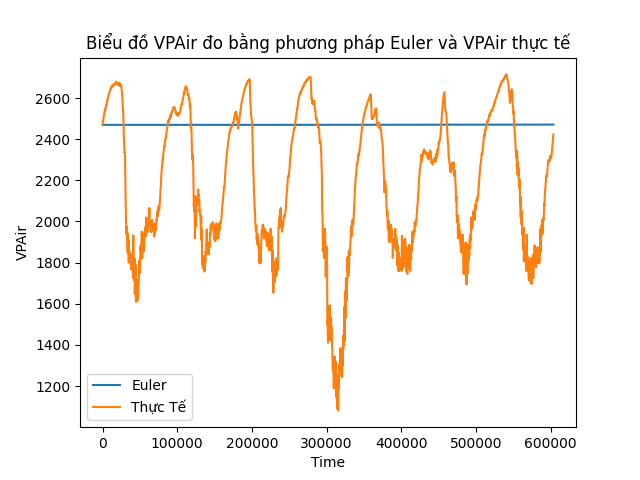
\includegraphics[width=7cm]{5b_euler.png}
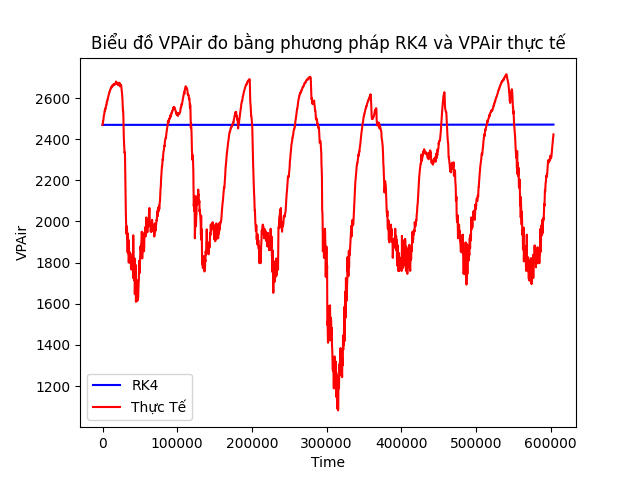
\includegraphics[width=7cm]{5b_rk4.png}
\end{center}
\end{figure}

\begin{figure}[h]
\begin{center}
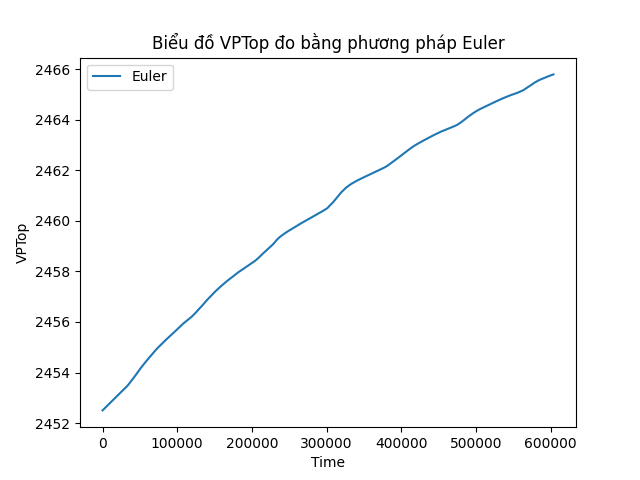
\includegraphics[width=7cm]{5b_TOP_Euler.png}
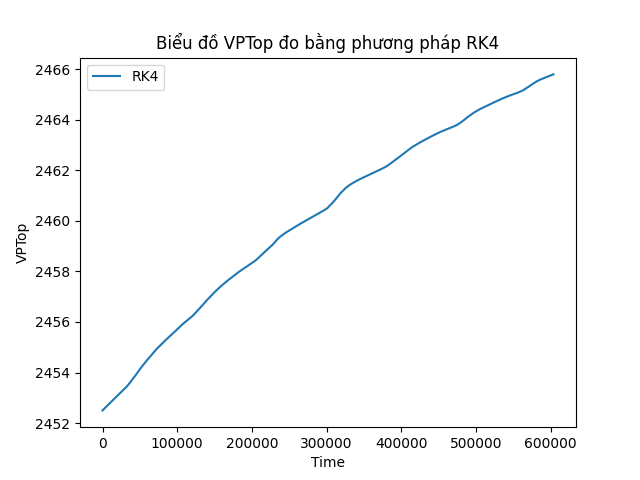
\includegraphics[width=7cm]{5b_TOP_RK4.png}
\end{center}
\end{figure}

\newpage

%%%%%%%%%%%%%%%%%%%%%%%%%%%%%%%%%
\begin{thebibliography}{80}


\bibitem{bib1}
\textbf{Link source code của nhóm: }
\url{https://github.com/phucvinh57/Mathematical_Modelling_Assignment}


\end{thebibliography}
\end{document}

